\chapter{Война}

\begin{figure}[H]
  \centering
  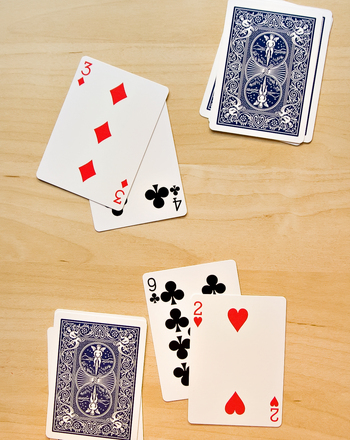
\includegraphics[width=1.0\linewidth,height=0.5\linewidth]{fig100001.png}
  \caption{„Война“ \\ https://images.squarespace-cdn.com/content/v1/59ea6080a803bb2f70ecbae5/1529350057743-92YH5Y0BN0JUMYB6X7NV/close-call-slide.jpg}
\label{fig100001}
\end{figure}

Играта „Война“ (Фиг. \ref{fig100001}) е детска игра с карти, като в основния си вариант се играе от двама играчи. Картите са стандартни, 52 карти за игра. Боите на картите са равноправни и няма сила по цвят. Всяка карта има сила с която участва в играта, като се започва от двойките (2 точки) и се стига до асата (14 точки). Тестето карти се разбърква и се раздава по равно на двамата играчи. Картите са с лицата на долу, като на всеки ход всеки от играчите показва най-горната карта. Играчът с по-силна карта взема и двете карти. Ако картите са с еднаква сила, то това е „война“ и играчите показват по три карти. Войната се печели от играча с по-силна трета карта. Ако и третите карти съвпадат, войната продължава, докато единият играч загуби войната. Спечелилият играч прибира всички карти, обърнати с лицето нагоре. Прибраните карти винаги застават най-отдолу в тестето на съответния играч. Играта се губи от този играч, който остане без карти. 

\section{Оформяне на графичния интерфейс}

Играта е относително проста и не изисква специални умения, което я прави идеален вариант за малки деца. Работата по изработването на тази игра, под формата на мобилно приложение, започва със създаването на нов проект (Фиг. \ref{fig100002}).

\begin{figure}[H]
  \centering
  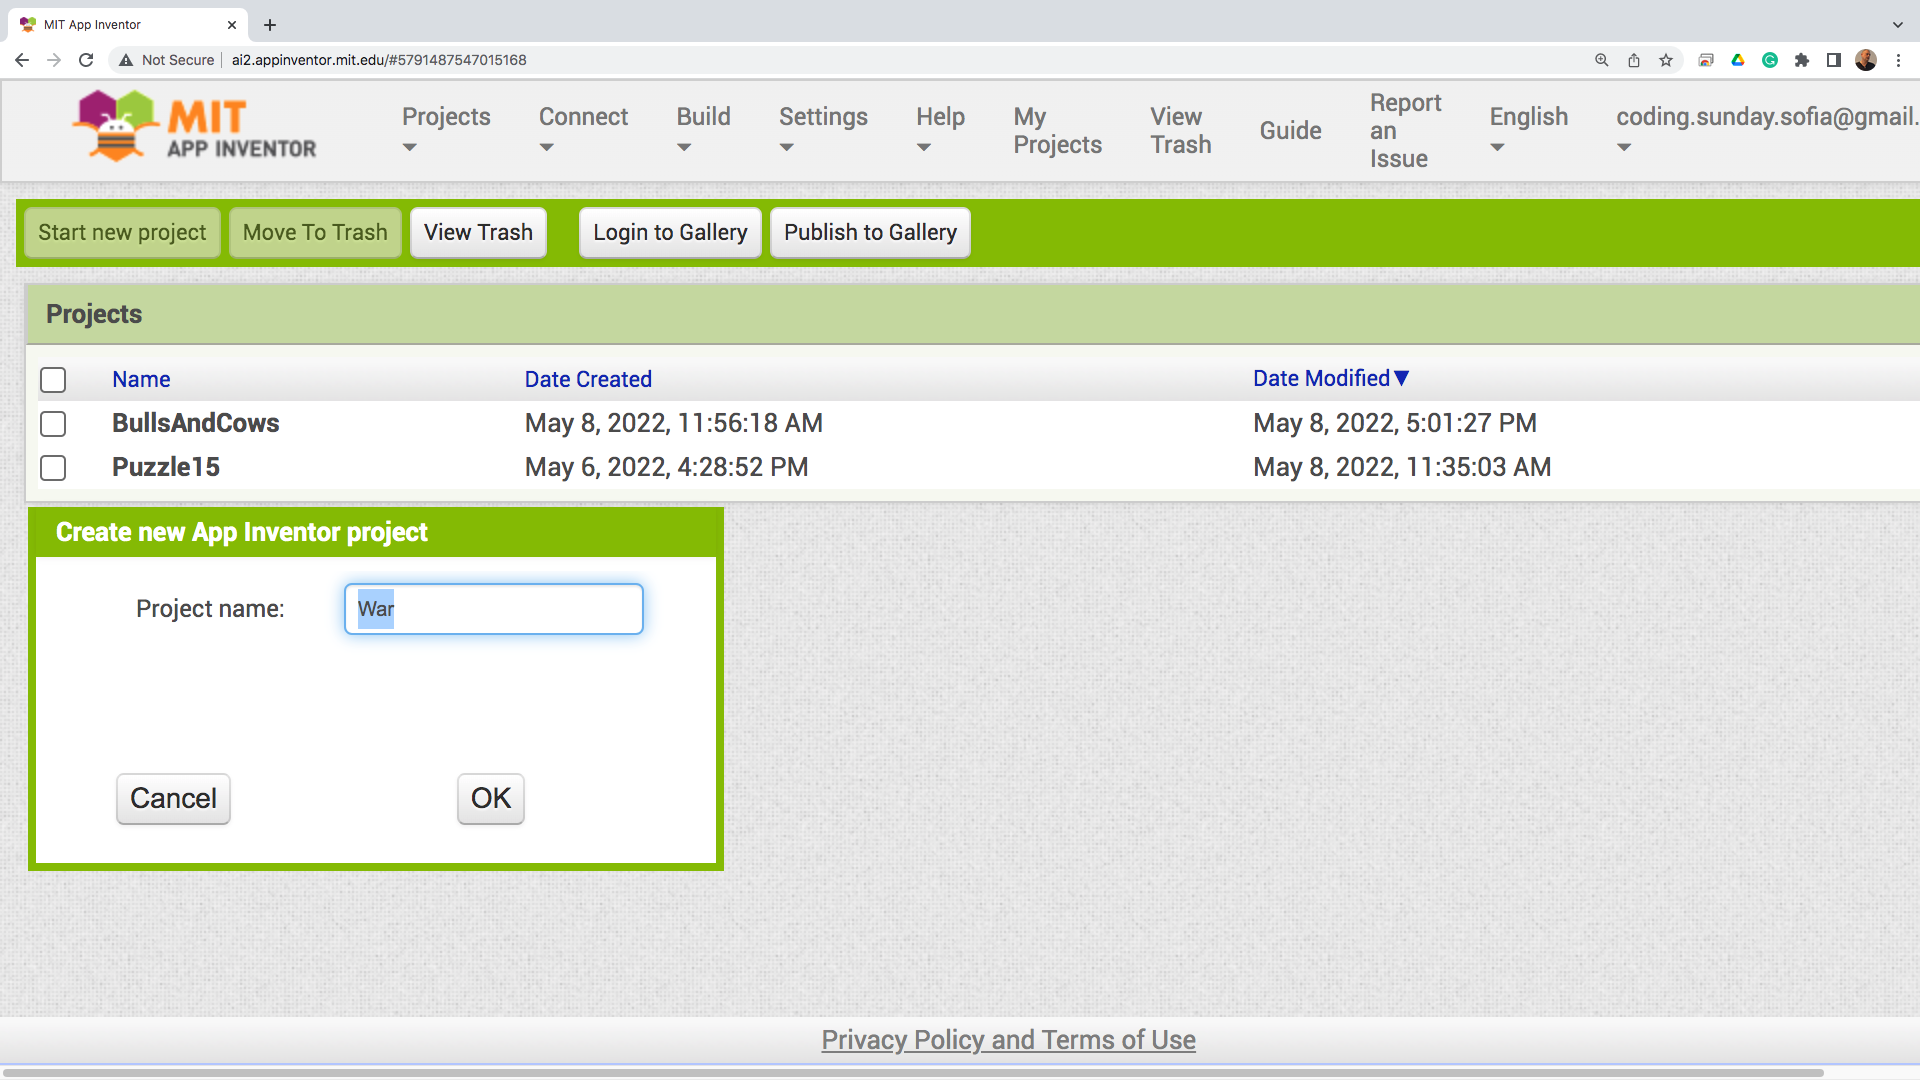
\includegraphics[width=1.0\linewidth,height=0.5\linewidth]{fig100002.png}
  \caption{Създаване на нов проект за играта „Война“}
\label{fig100002}
\end{figure}

Потребителският интерфейс ще бъде възможно най-опростен. Два бутона (Фиг. \ref{fig100003}), най-отгоре в работното пространство, ще служат за стартиране на нова игра и направата на ход.

\begin{figure}[H]
  \centering
  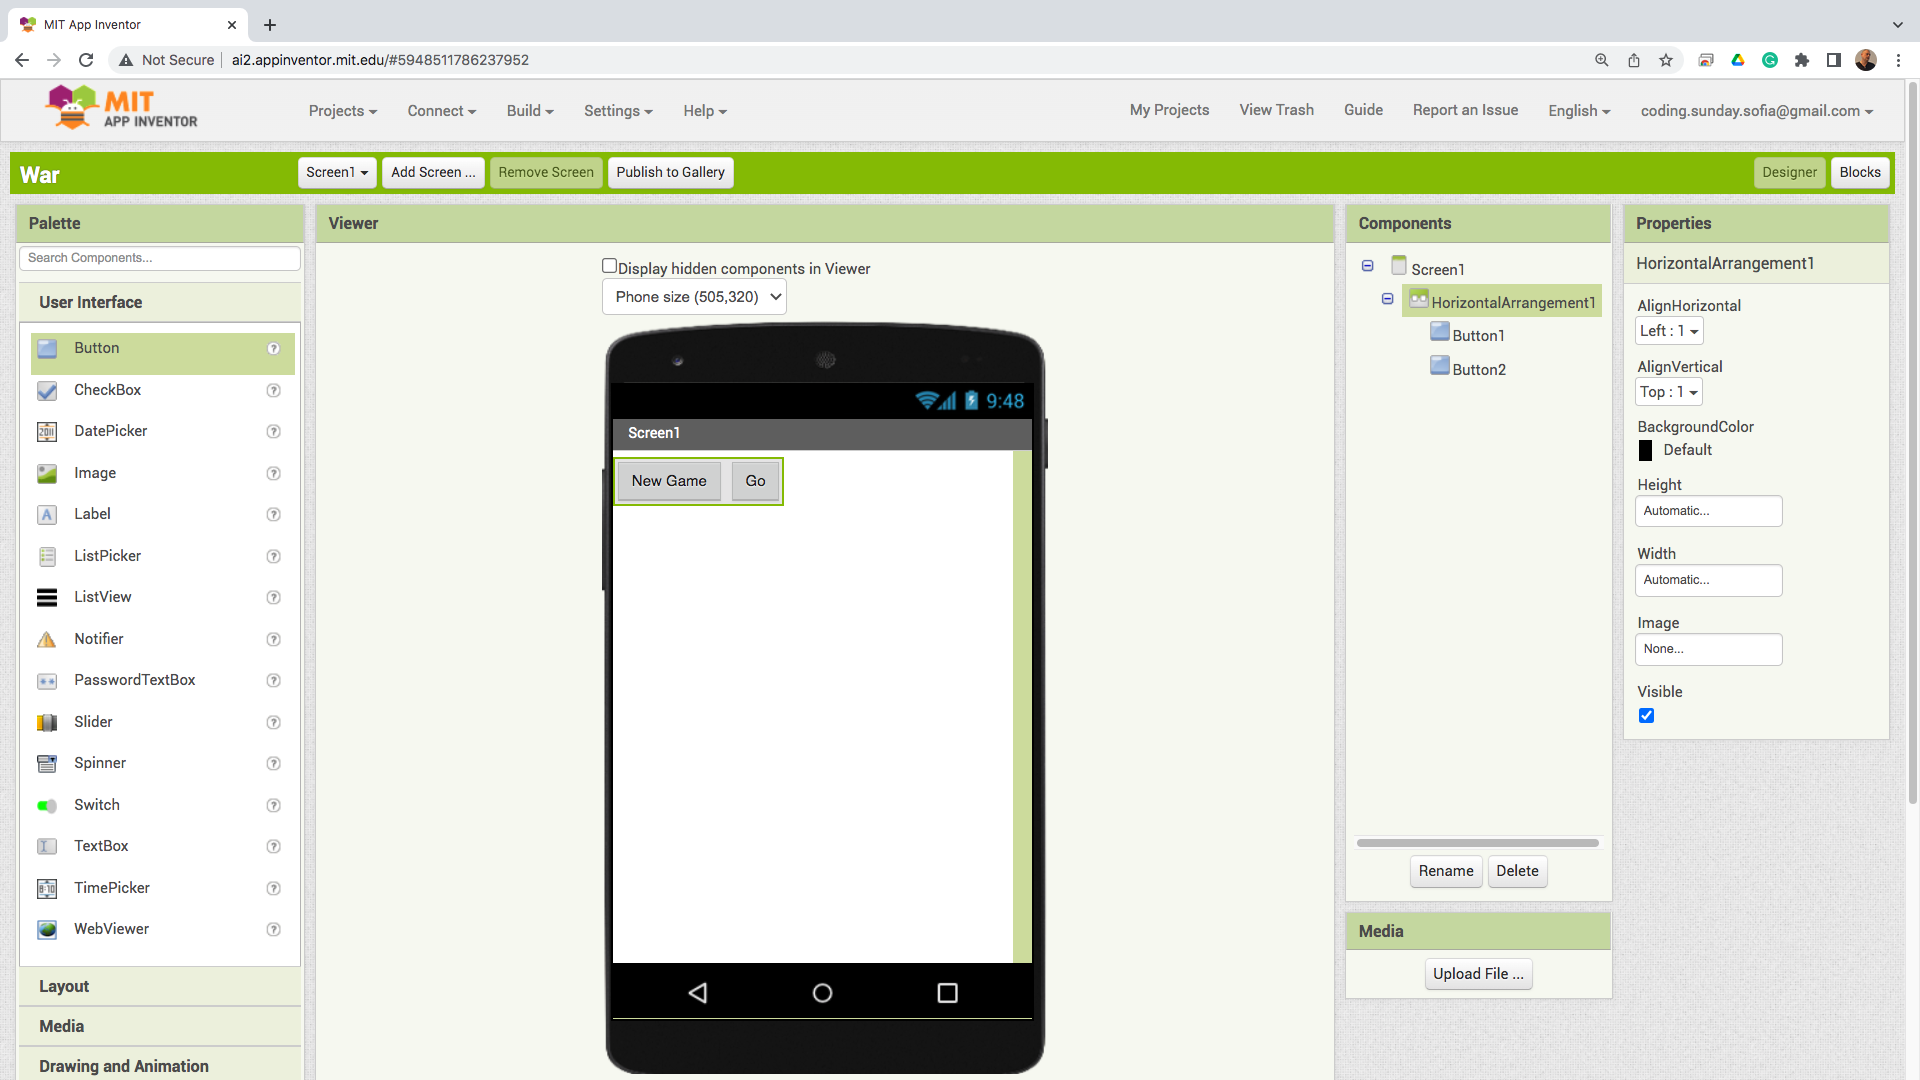
\includegraphics[width=1.0\linewidth,height=0.5\linewidth]{fig100003.png}
  \caption{Бутони за стартиране на нова игра и направа на ход}
\label{fig100003}
\end{figure}

Веднага под бутоните, в табличен вид се подреждат два реда с визуални компоненти за показване на графични изображения (Фиг. \ref{fig100004}). В първата колона ще се визуализира гръб на карта, което символизира тестетата на двамата играчи, а в другите три съседни компонента ще се показва една карта, когато няма война и три карти, когато има война. 

\begin{figure}[H]
  \centering
  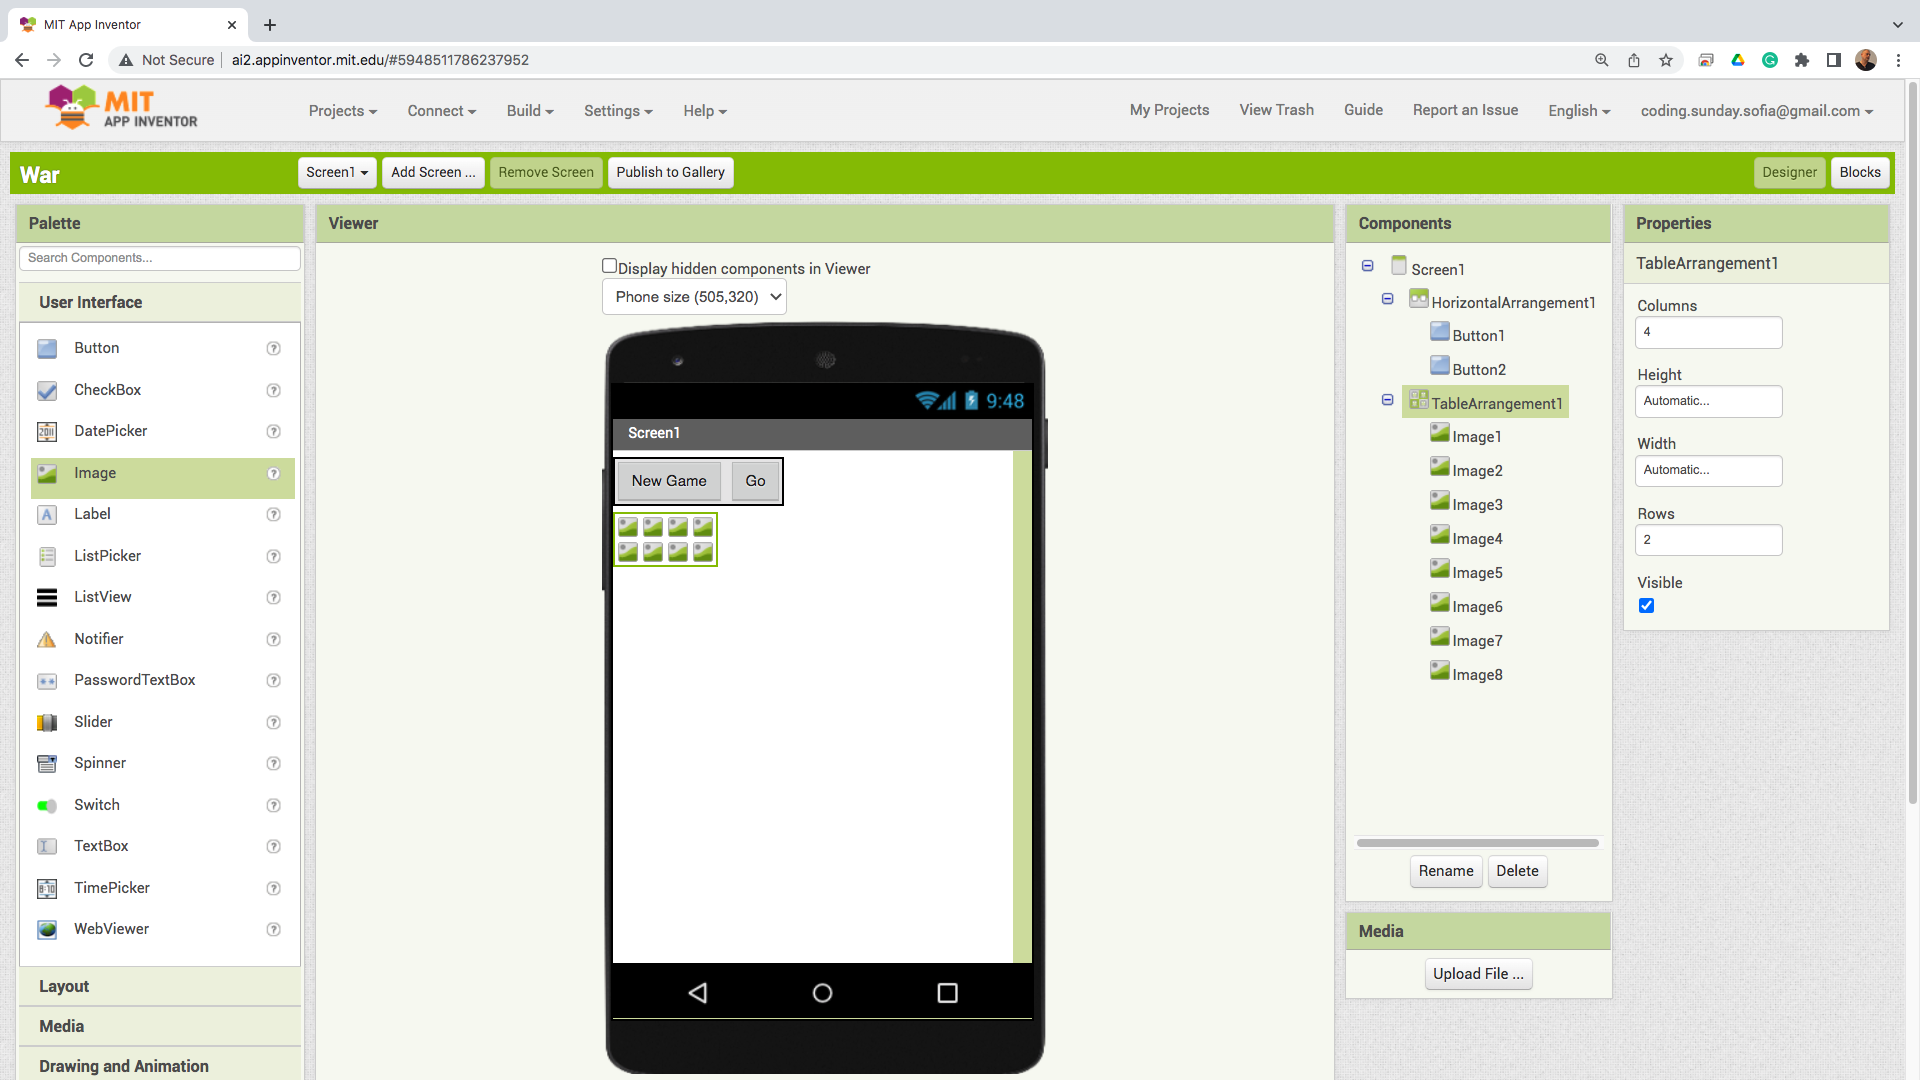
\includegraphics[width=1.0\linewidth,height=0.5\linewidth]{fig100004.png}
  \caption{Компоненти за визуализация на картите}
\label{fig100004}
\end{figure}

За изображенията на самите карти може да се използва всеки комплект от карти, които се разпространяват със свободен лиценз за не търговска употреба (Фиг. \ref{fig100005}).

\begin{figure}[H]
  \centering
  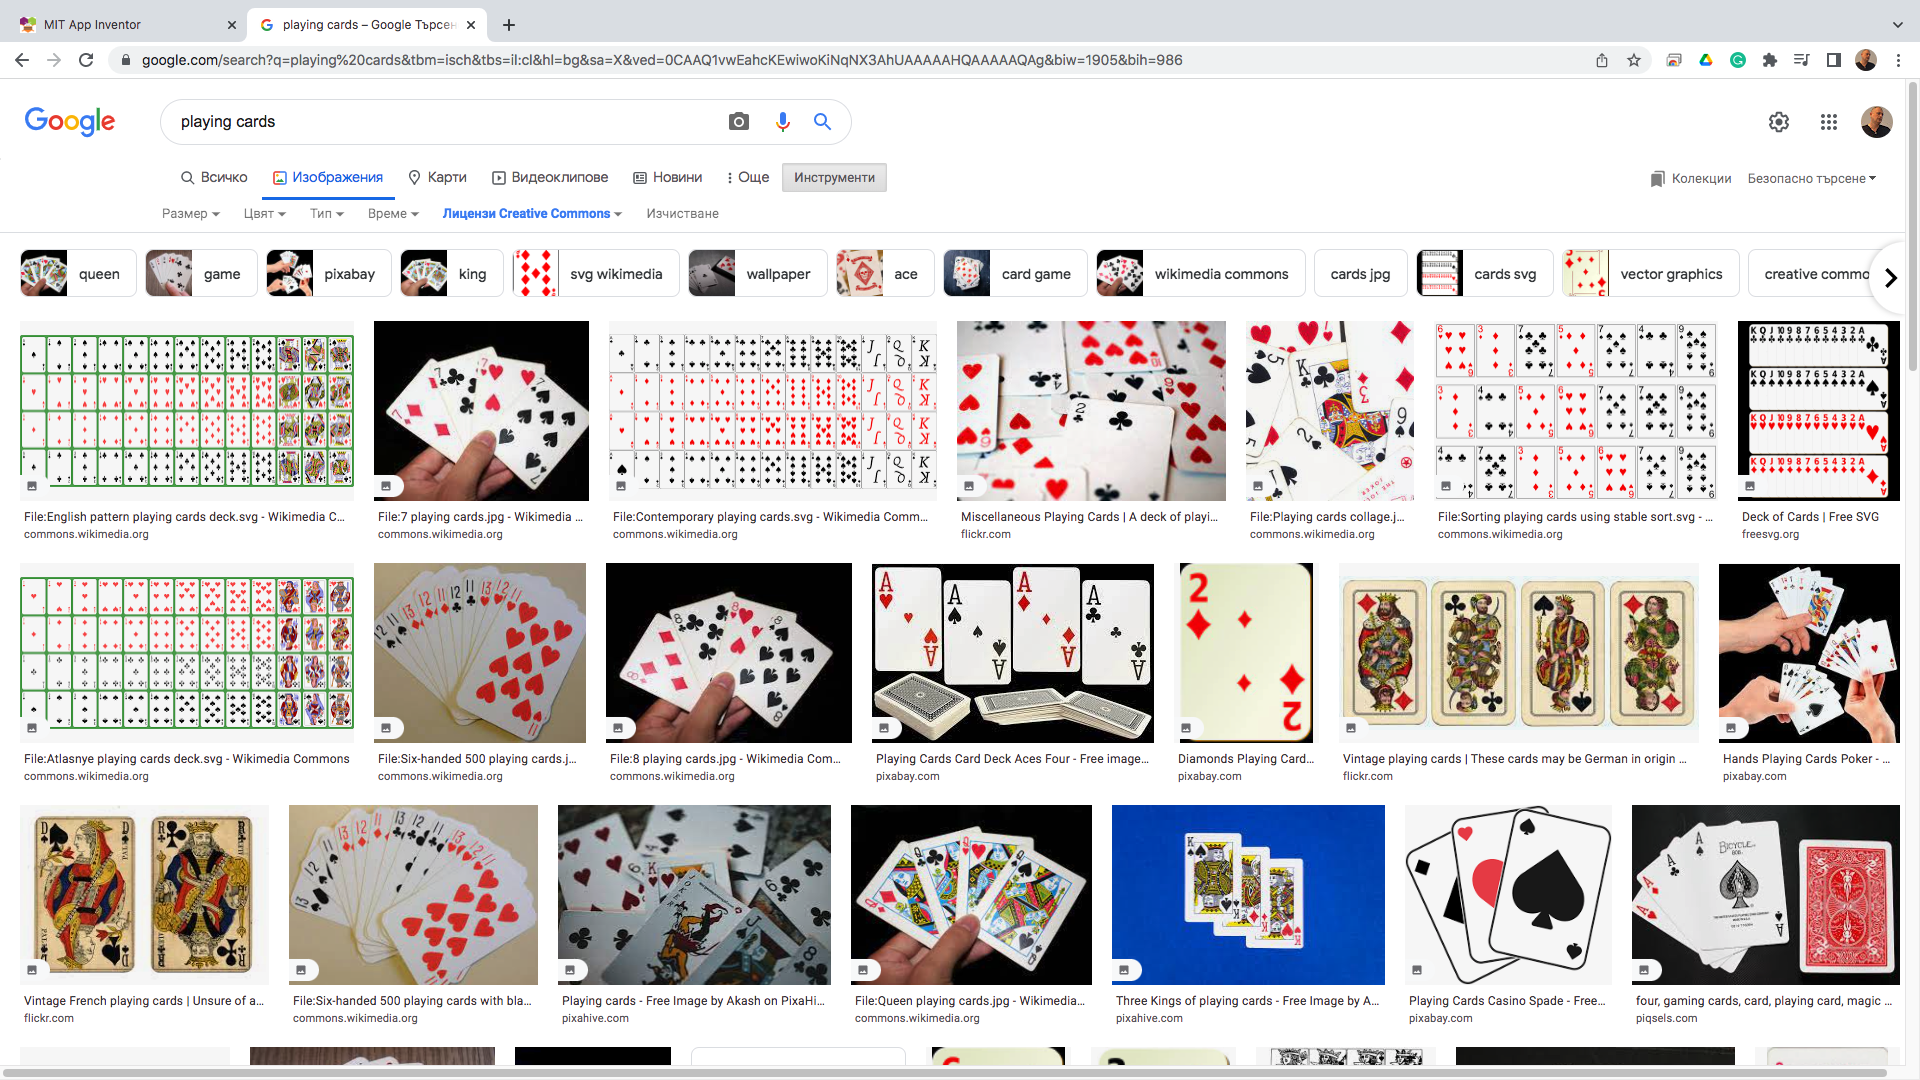
\includegraphics[width=1.0\linewidth,height=0.5\linewidth]{fig100005.png}
  \caption{Изображения на карти за игра}
\label{fig100005}
\end{figure}

Ако комплектът карти е в общо изображение, то се нарязва на 52 отделни изображения и поне едно изображение за гръб на картите. Така подготвените 53 графични файла, се зареждат в проекта, като се качват файл по файл (Фиг. \ref{fig100006}).

\begin{figure}[H]
  \centering
  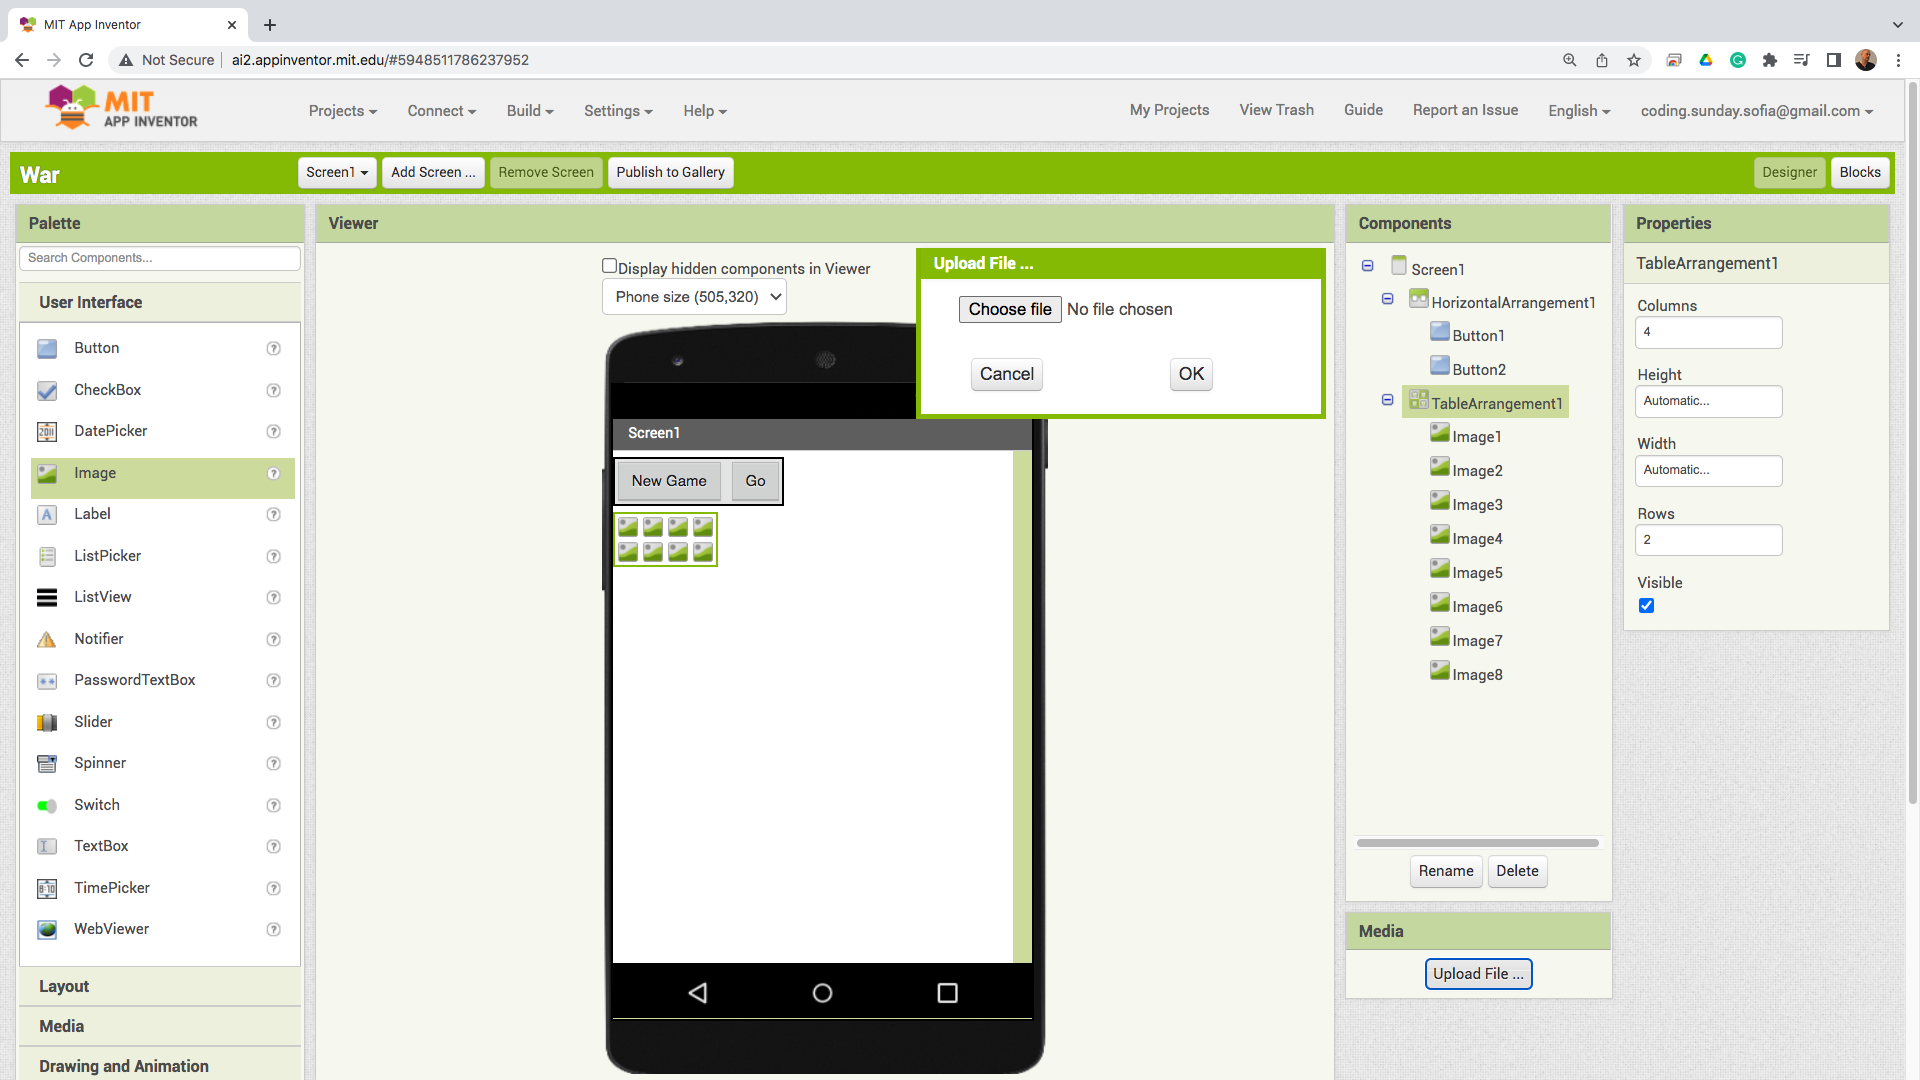
\includegraphics[width=1.0\linewidth,height=0.5\linewidth]{fig100006.png}
  \caption{Качване на графични файлове}
\label{fig100006}
\end{figure}

От така качените графични файлове, в първата колона от изображения се зарежда изображението за гръб на картите (Фиг. \ref{fig100007}).

\begin{figure}[H]
  \centering
  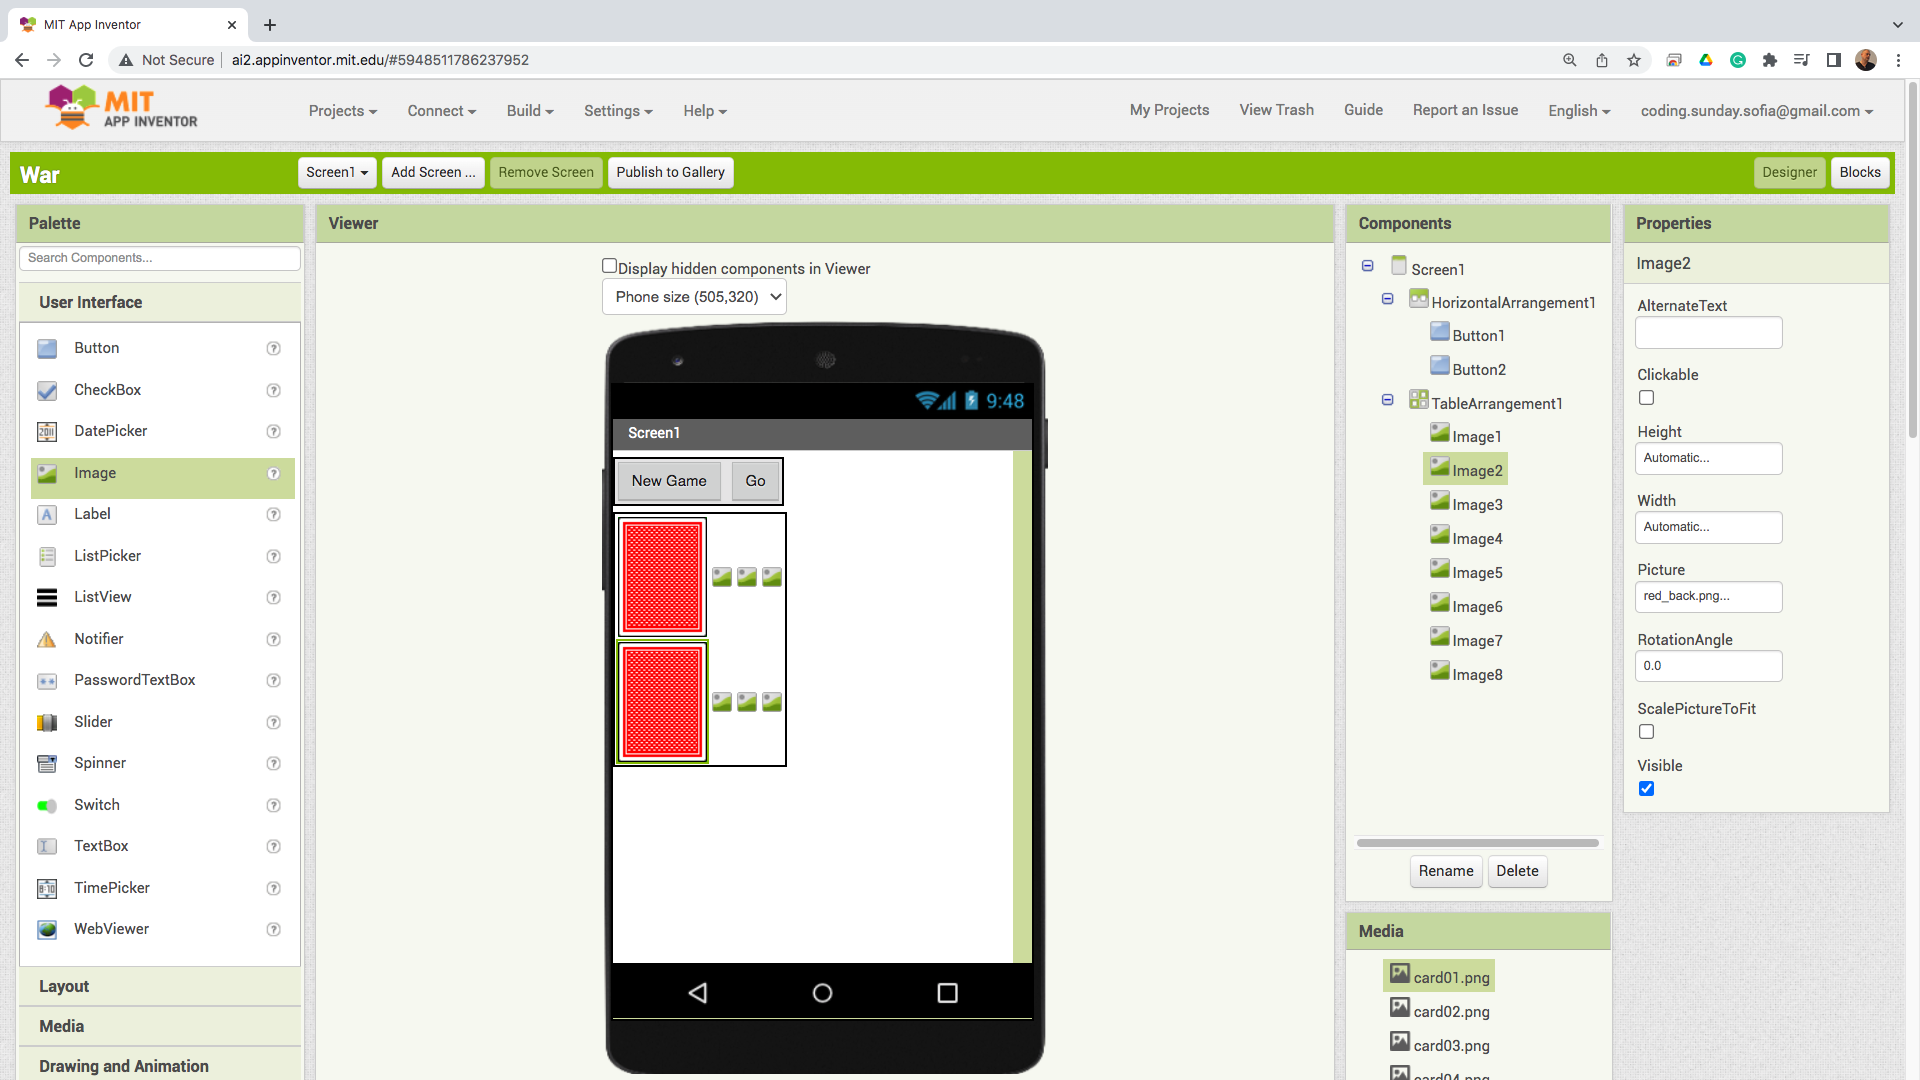
\includegraphics[width=1.0\linewidth,height=0.5\linewidth]{fig100007.png}
  \caption{Изображения за маркирането на тестетата}
\label{fig100007}
\end{figure}

\section{Използване на структури от данни}

Картите ще циркулират в модела на играта под формата на цели числа. За тази цел се обявяват пет помощни, глобални променливи - списък с основното тесте, два списъка за картите държани от играча и два списъка за картите поставени на масата от играчите (Фиг. \ref{fig100008}). 

\begin{figure}[H]
  \centering
  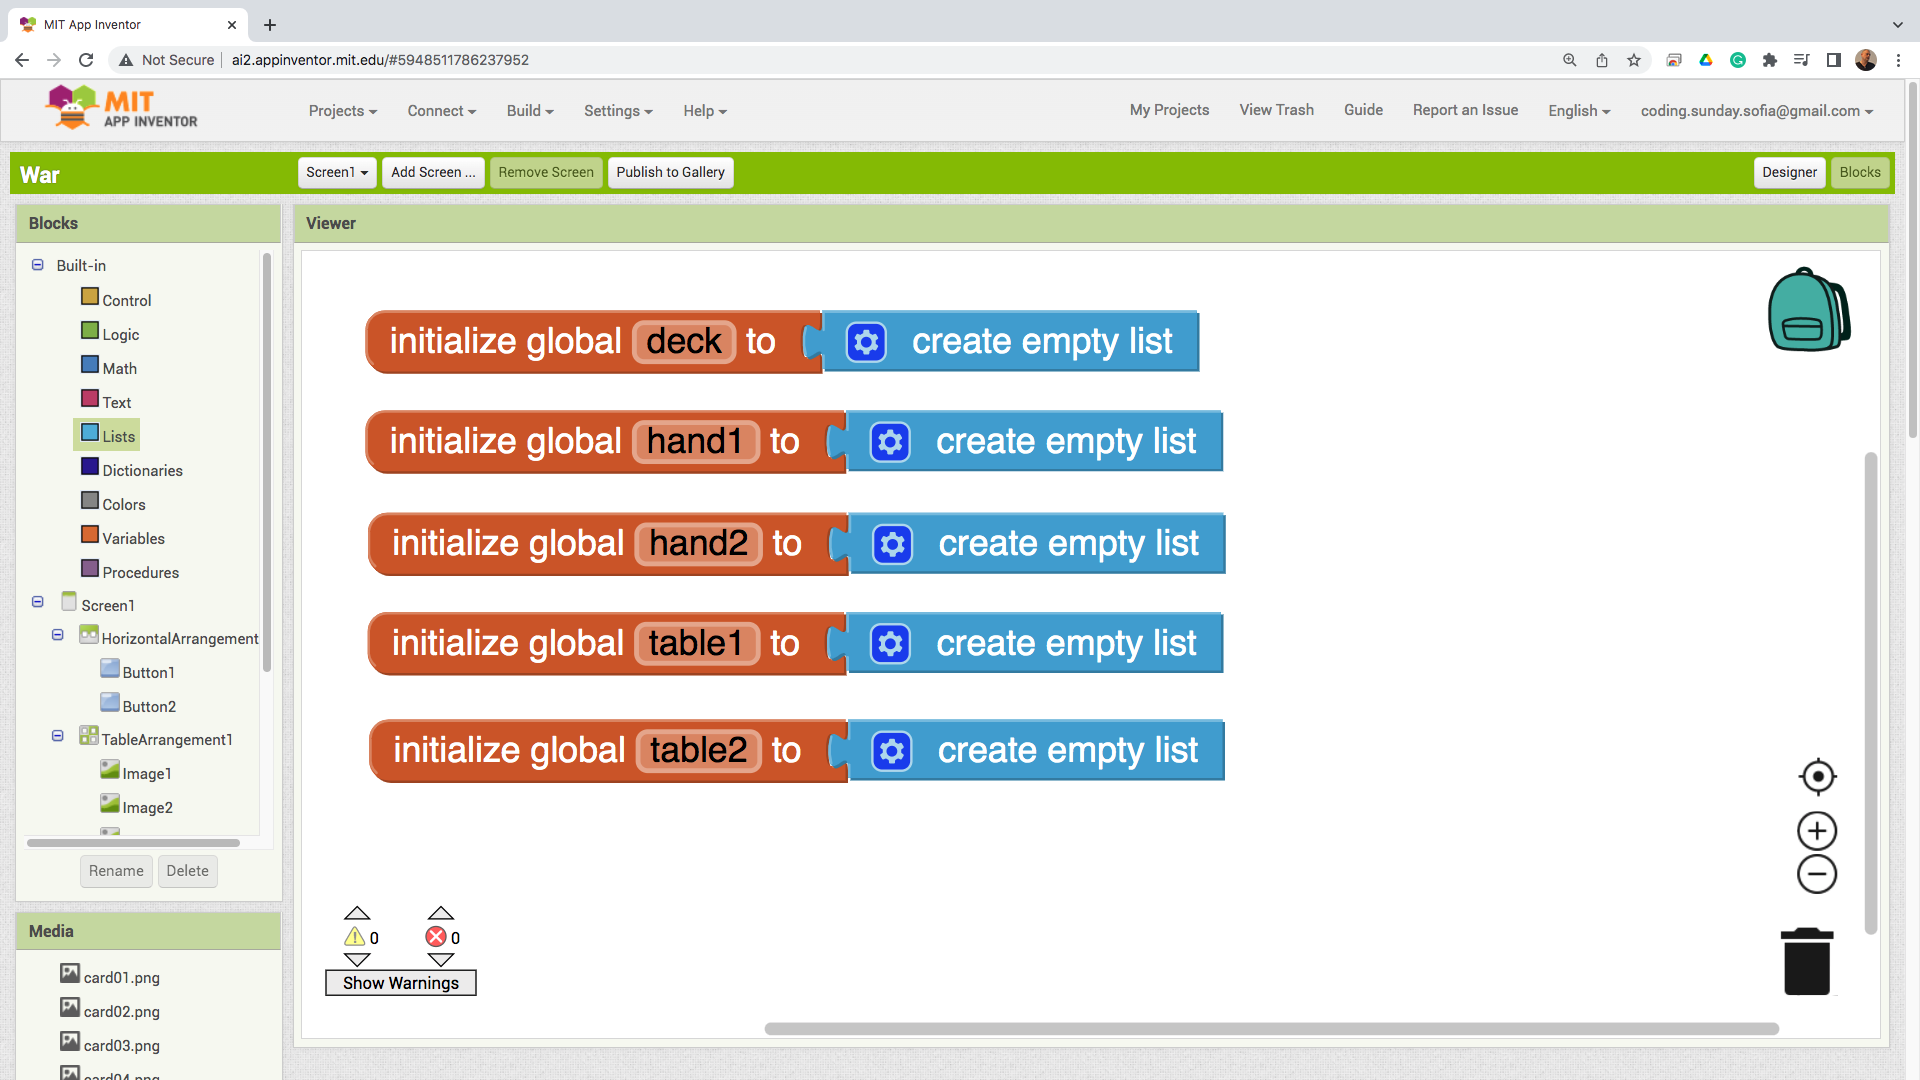
\includegraphics[width=1.0\linewidth,height=0.5\linewidth]{fig100008.png}
  \caption{Основни помощни променливи}
\label{fig100008}
\end{figure}

Два допълнителни списъка биха улеснили визуализацията на картите, които се поставят на масата. В тези списъци се поместват отпратки към визуалните компоненти за показване на изображения (Фиг. \ref{fig100009}).

\begin{figure}[H]
  \centering
  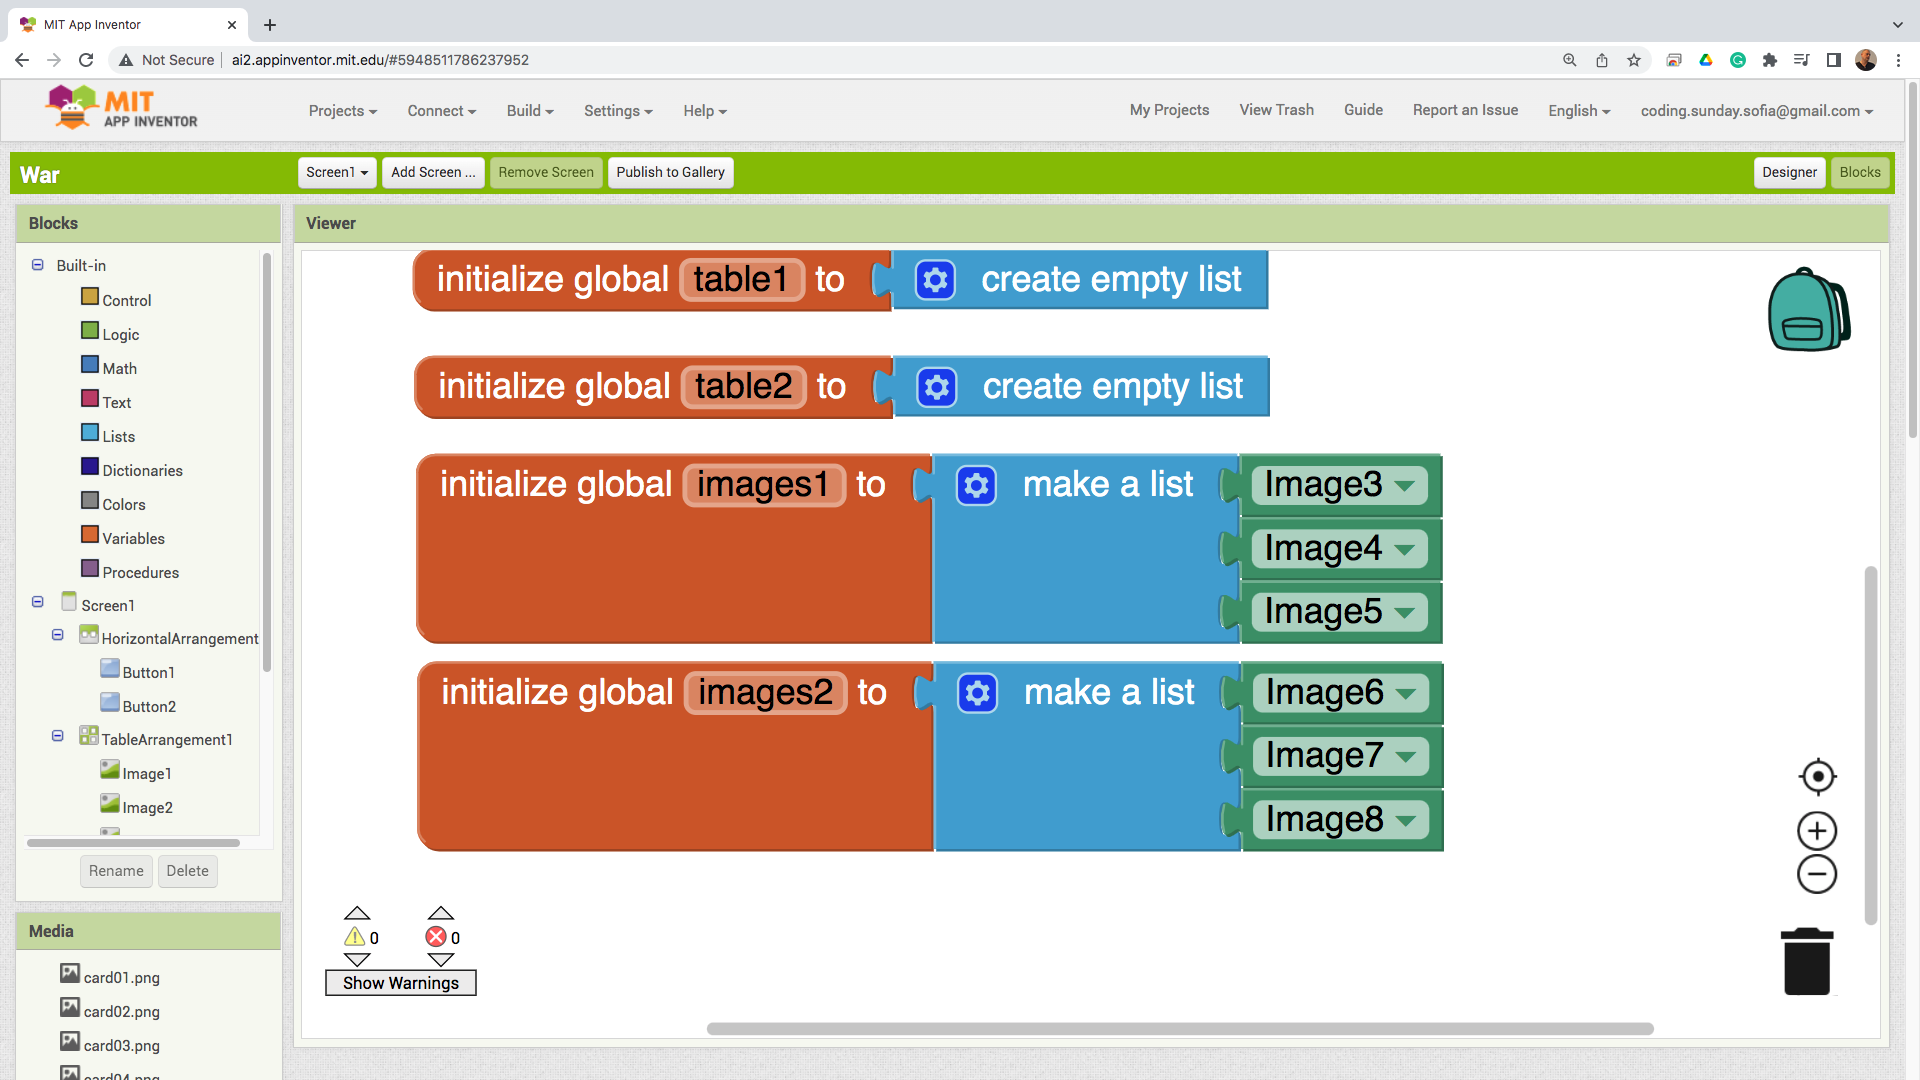
\includegraphics[width=1.0\linewidth,height=0.5\linewidth]{fig100009.png}
  \caption{Помощни списъци за визуализация}
\label{fig100009}
\end{figure}

Последната помощна променлива подрежа в списък изображенията на картите. Подредбата е важна, като двойките стоят на първите четири места, на вторите четири места стоят тройките и така нататък, докато се стигне до последните четири места на които стоят асата (Фиг. \ref{fig100010}). Благодарение на тази подредба, при пресмятането на победителите в отделните рундове ще се постига с просто аритметично пресмятане. 

\begin{figure}[H]
  \centering
  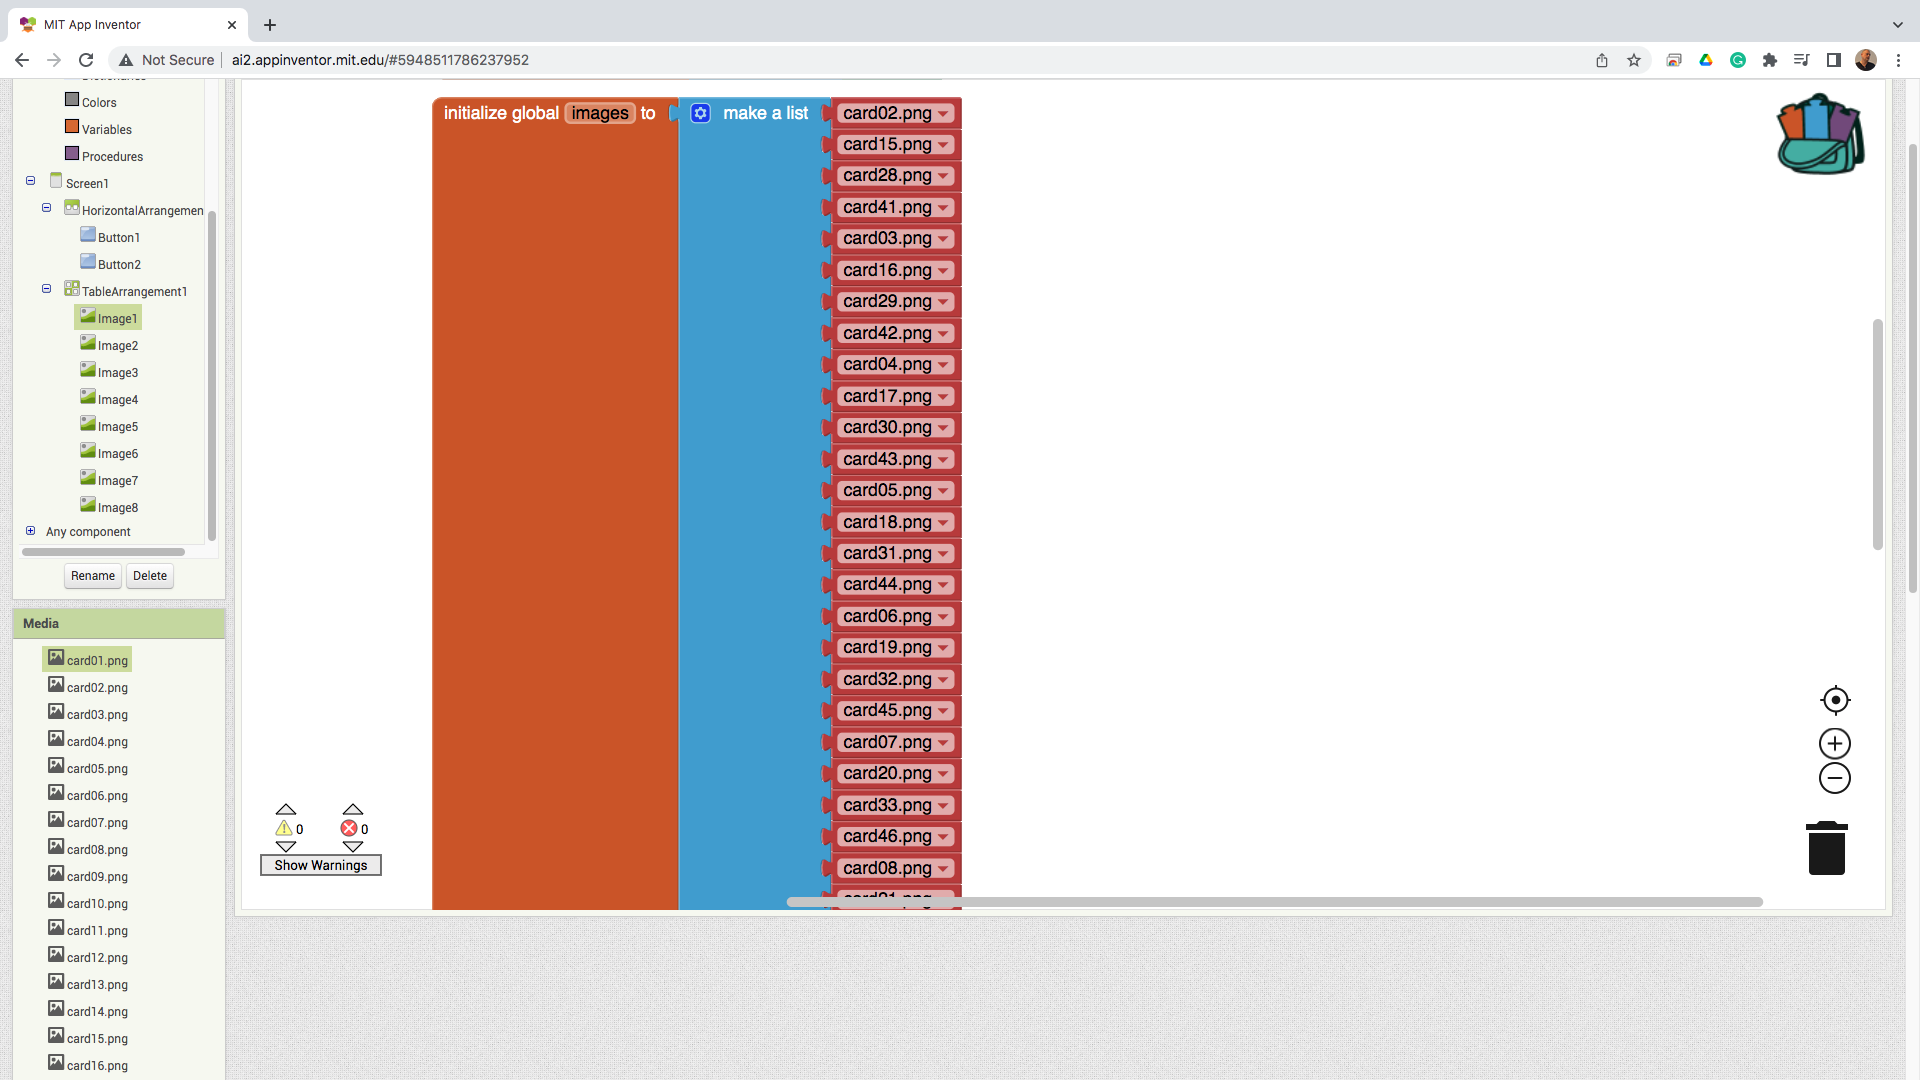
\includegraphics[width=1.0\linewidth,height=0.5\linewidth]{fig100010.png}
  \caption{Помощна променлива за реда на картите по сила}
\label{fig100010}
\end{figure}

\section{Алгоритми за манипулация на структурите в играта}

Започването на играта е свързано с правилно организиране на отделните списъци. Като начало, всички помощни списъци трябва да бъдат инициализирани с празна стойност, така че да не премине паразитна информация от предишни разигравания. За тази цел най-удачно може да се постигне с помощна функция (Фиг. \ref{fig100011}).

\begin{figure}[H]
  \centering
  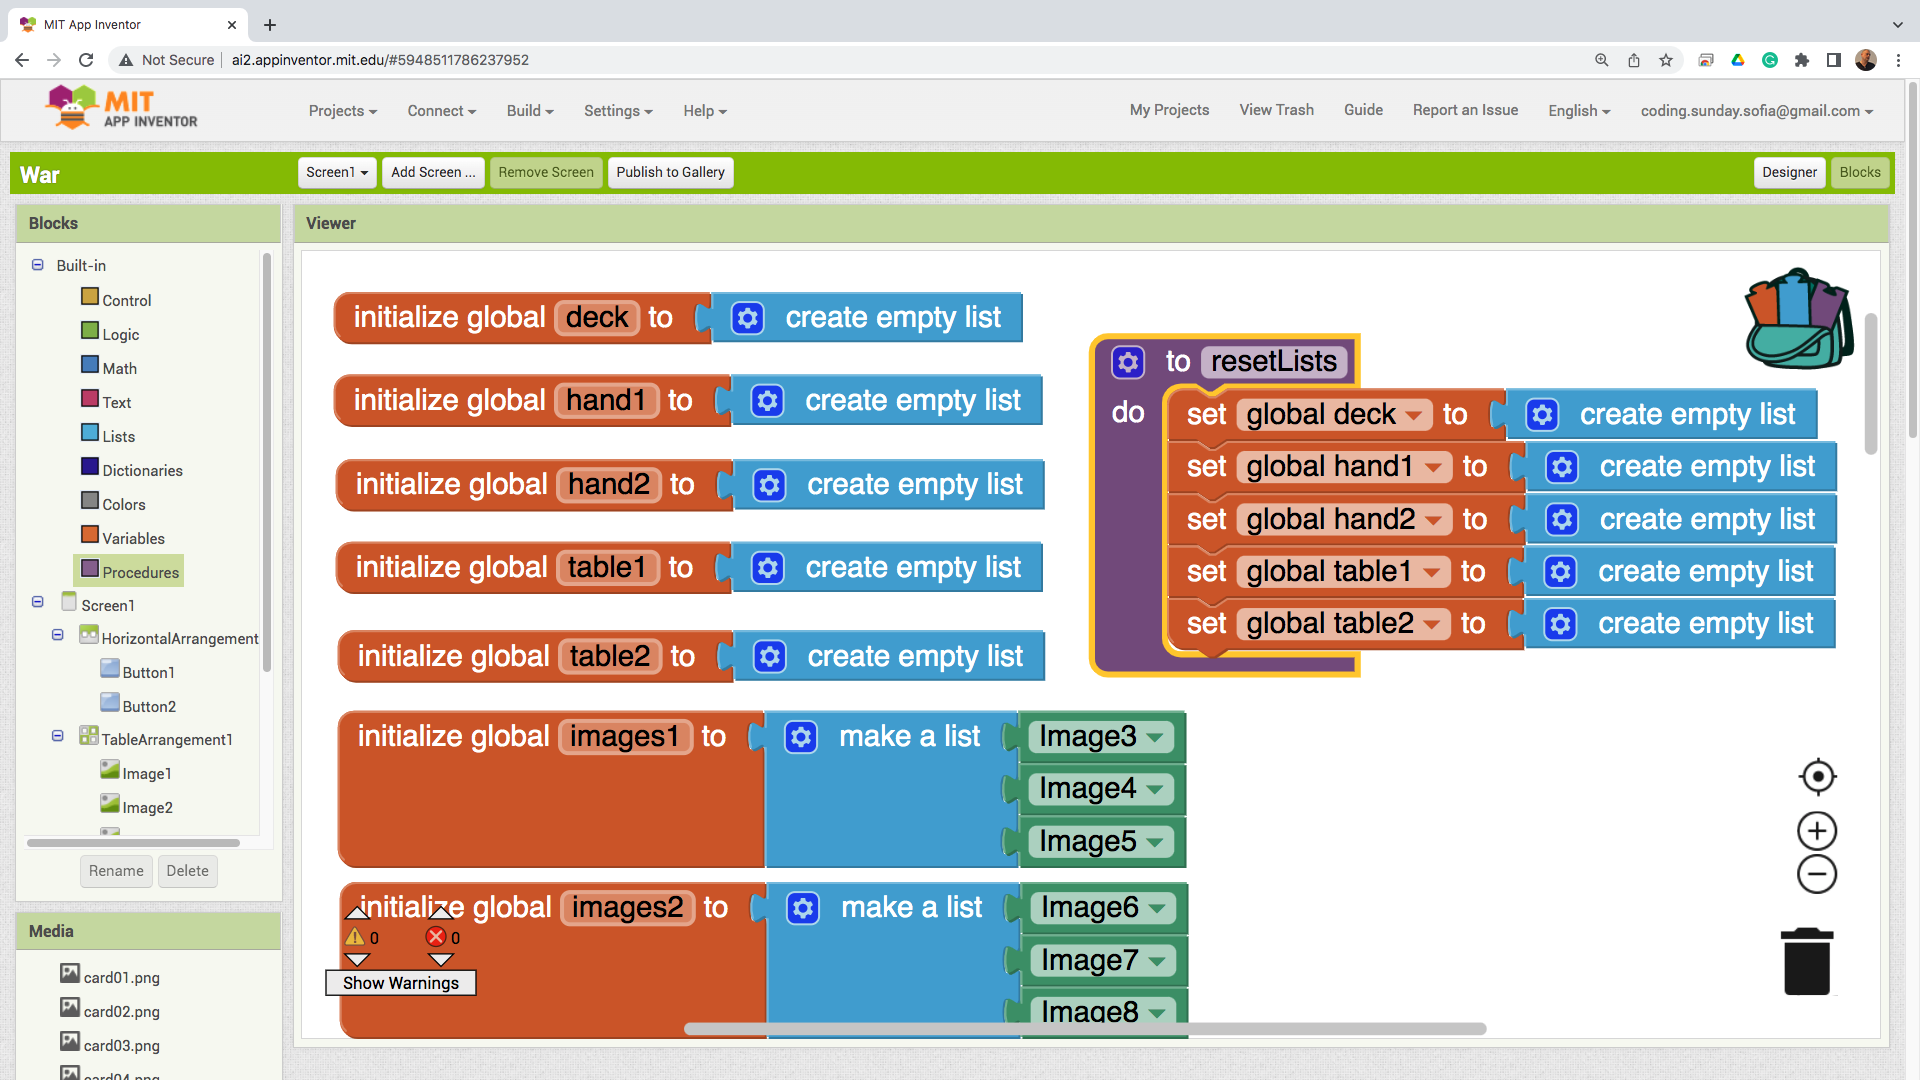
\includegraphics[width=1.0\linewidth,height=0.5\linewidth]{fig100011.png}
  \caption{Инициализация на празни списъци}
\label{fig100011}
\end{figure}

Основното тесте карти съдържа в разбъркан вид числата от 1 до 52. Всяко от тези числа е индексът на съответната карта в помощния списък с изображенията на картите. За да се попълни основното тесте се завърта цикъл (Фиг. \ref{fig100012}) и индексът на цикъла се записва в случайно избрана позиция. Вмъкването на случаен елемент може да стане, като се генерира случайно число за индексът на вмъкване. Това случайно число трябва да е в диапазон от 1 до текущия размер на списъка. Когато списъкът е празен той има размер 0. В тази ситуация случайното число би било 0 или 1. Индексите в списъците не могат да бъдат 0 и поради тази причина е нужно допълнително, подсигуряващо блокче за максимална стойност между случайно генерираното число и числото 1.

\begin{figure}[H]
  \centering
  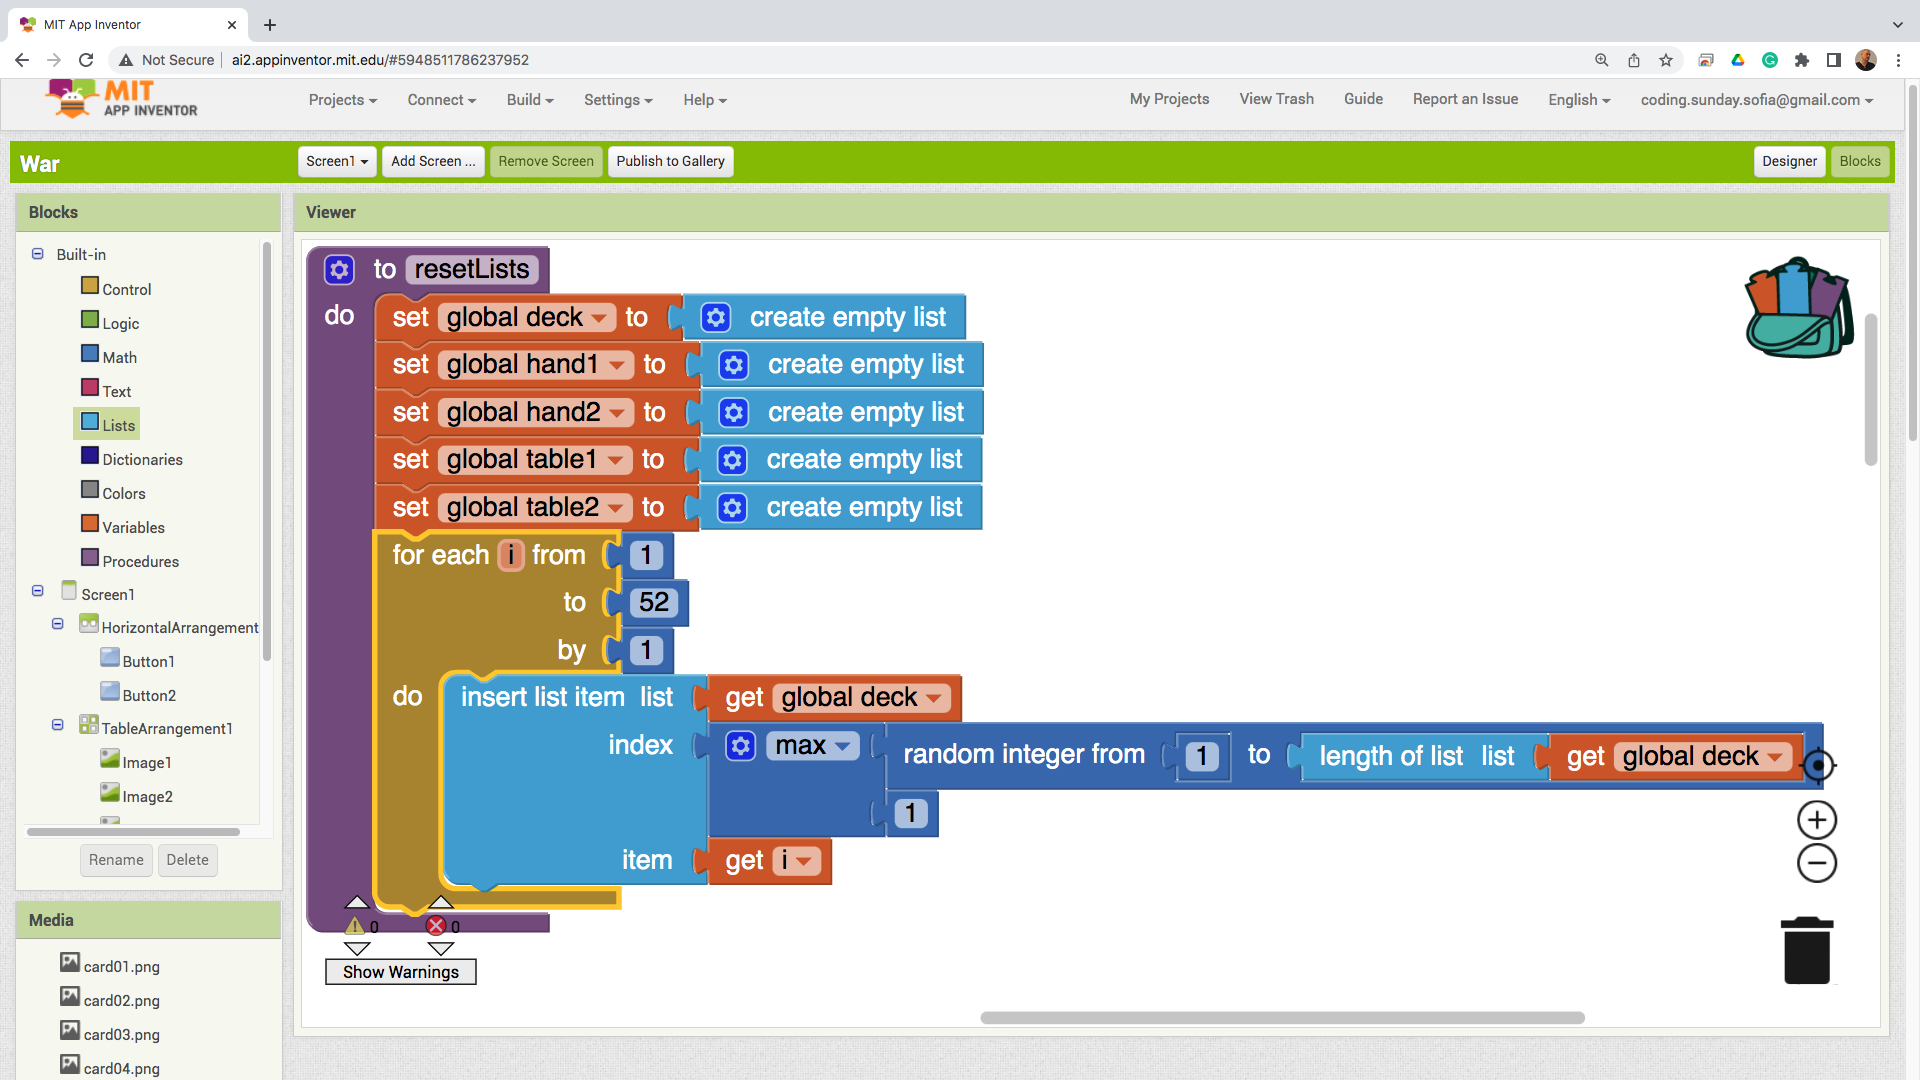
\includegraphics[width=1.0\linewidth,height=0.5\linewidth]{fig100012.png}
  \caption{Цикъл за инициализация на дека}
\label{fig100012}
\end{figure}

След като се получи разбъркването на основното тесте, следва раздаването на картите за двамата играчи. Всеки играч получава половината карти от основното тесте и те се записват в два от помощните списъци (Фиг. \ref{fig100013}). Стъпката в този цикъл е 2, тъй като четните карти отиват при единия играч, а нечетните карти отиват при другия играч. 

\begin{figure}[H]
  \centering
  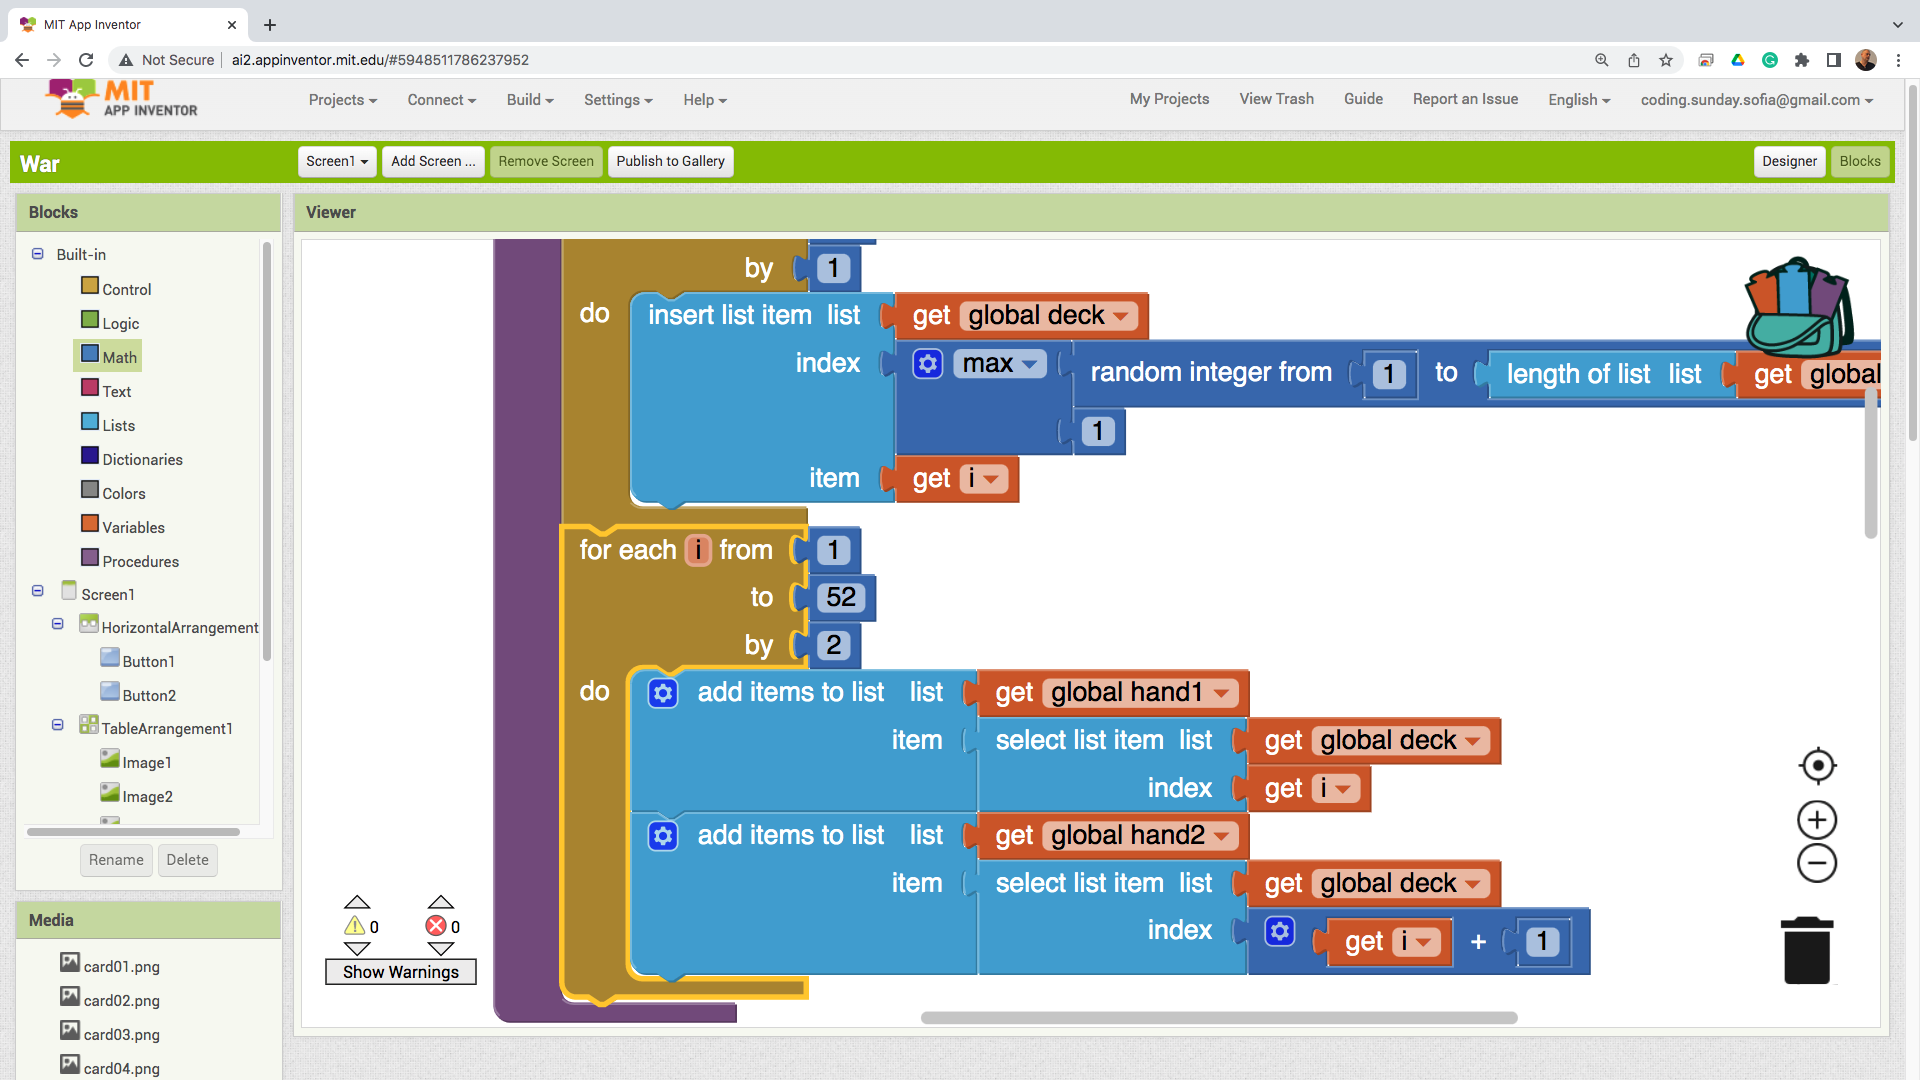
\includegraphics[width=1.0\linewidth,height=0.5\linewidth]{fig100013.png}
  \caption{Раздаване на картите}
\label{fig100013}
\end{figure}

След като картите бъдат раздадени, може да се приеме че основното тесте е празно (Фиг. \ref{fig100014}). 

\begin{figure}[H]
  \centering
  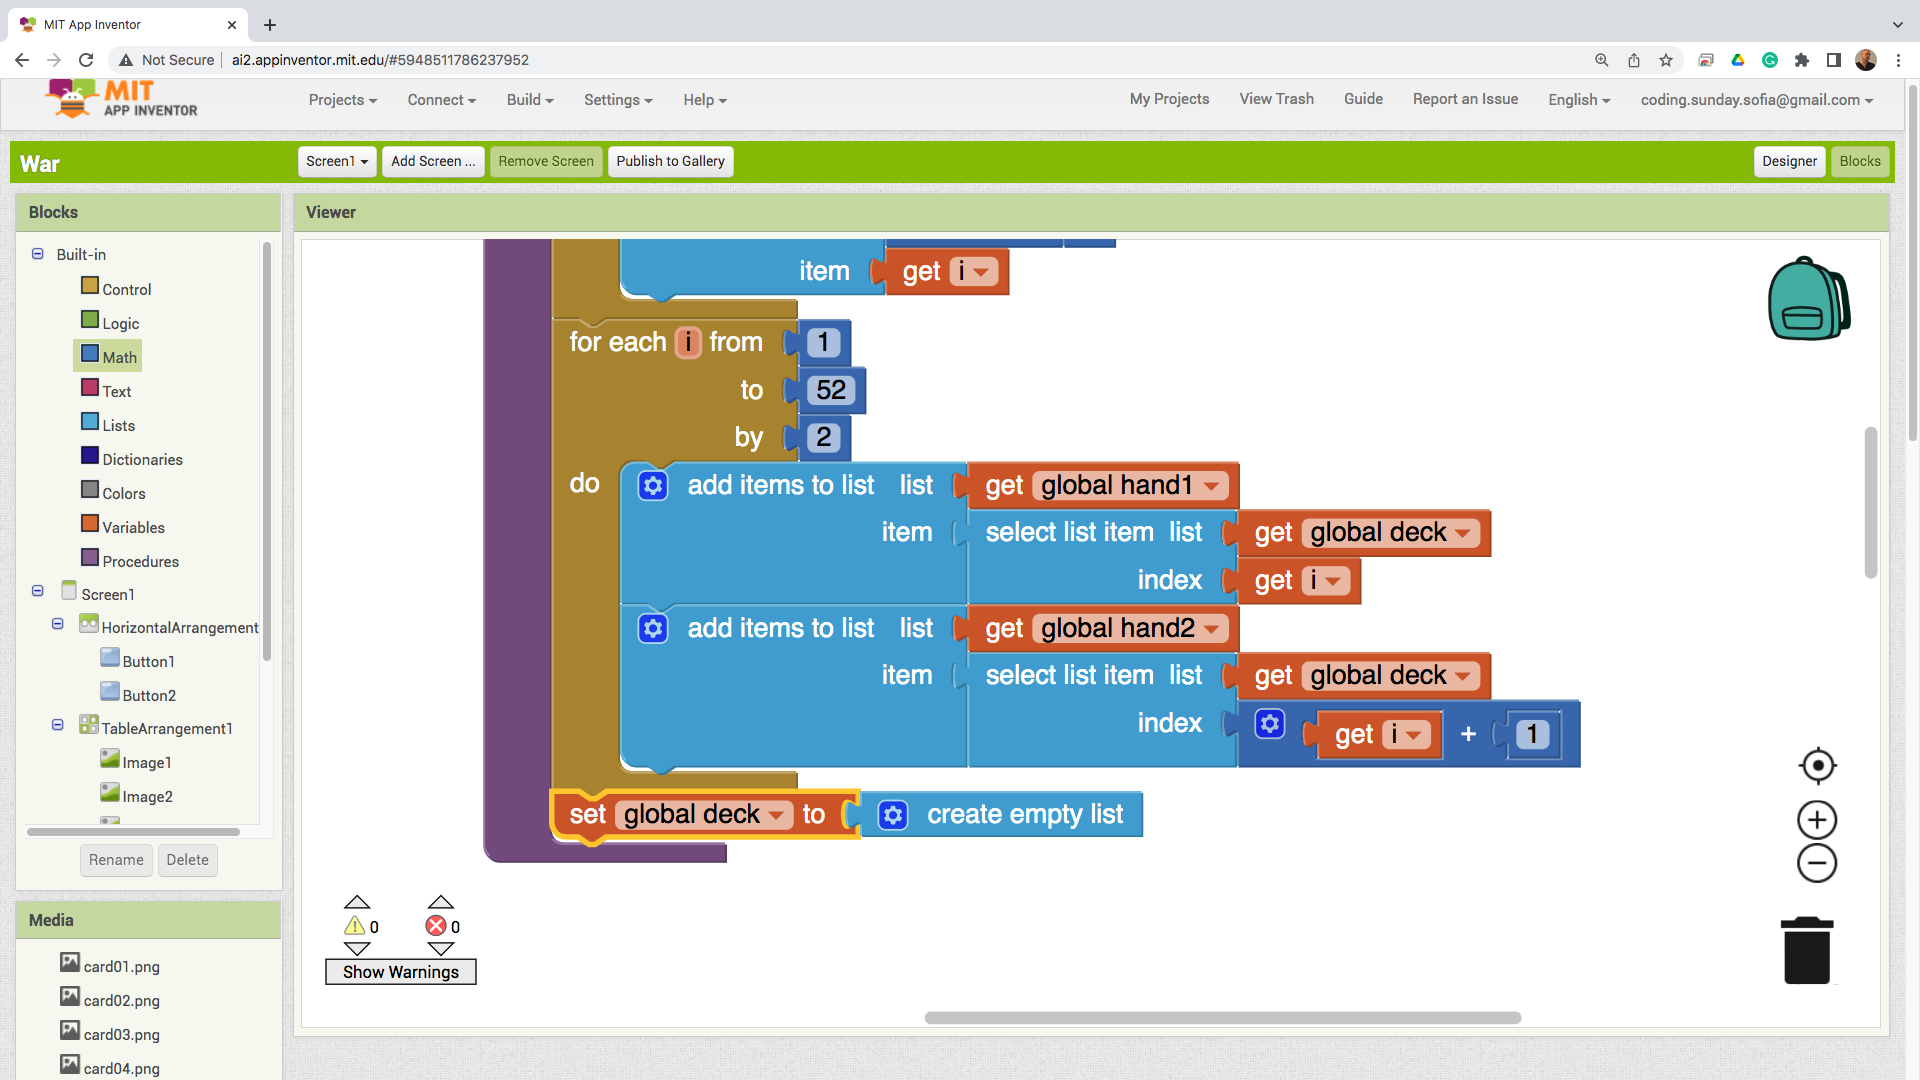
\includegraphics[width=1.0\linewidth,height=0.5\linewidth]{fig100014.png}
  \caption{Нулиране на дека}
\label{fig100014}
\end{figure}

В две ситуации е необходимо вътрешните структури да се инициализират – когато се стартира приложението и когато потребителят реши да започне нова игра (Фиг. \ref{fig100015}).

\begin{figure}[H]
  \centering
  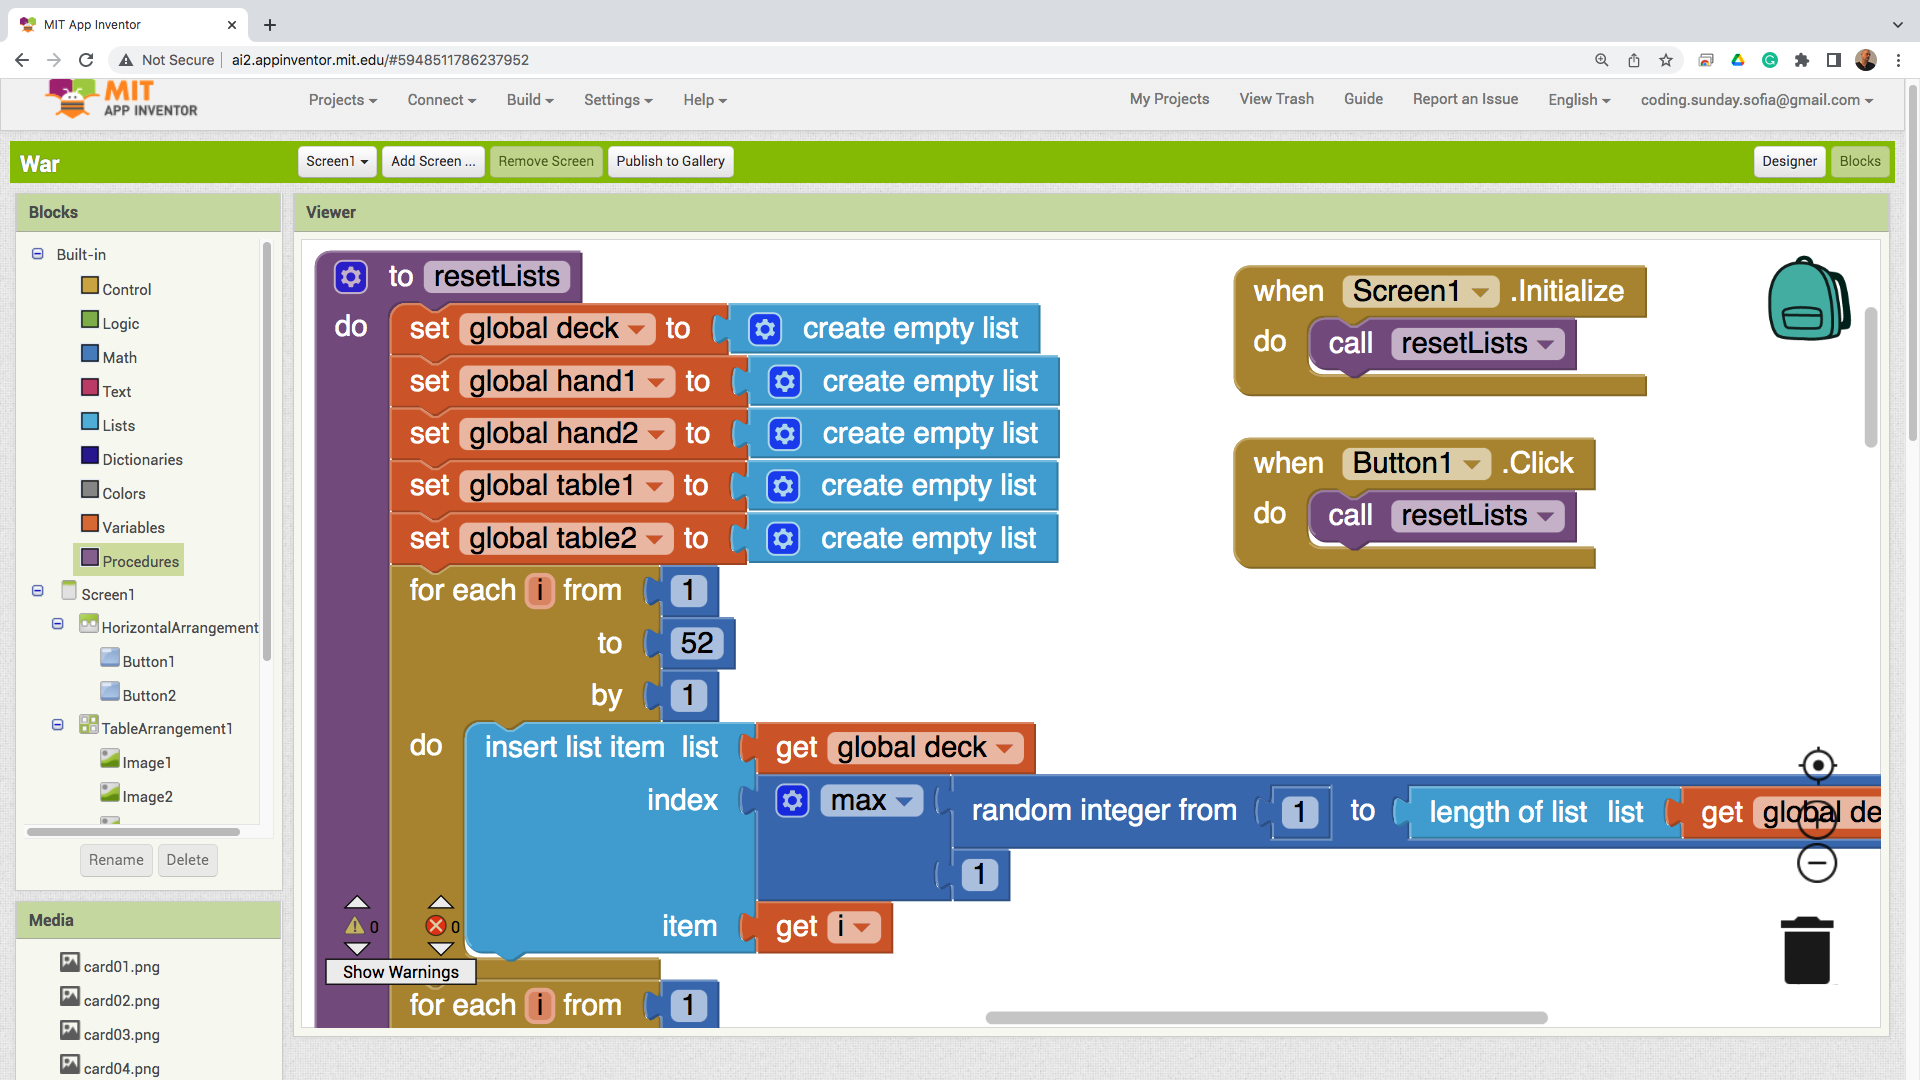
\includegraphics[width=1.0\linewidth,height=0.5\linewidth]{fig100015.png}
  \caption{Извиквания за инициализация}
\label{fig100015}
\end{figure}

Следващата помощна процедура премахва изображения, ако те са заредени в компонентите за визуализация на картинки (Фиг. \ref{fig100016}). Тази процедура е полезна при всеки ход, когато вече е уточнено кой играч ще събере картите от масата.

\begin{figure}[H]
  \centering
  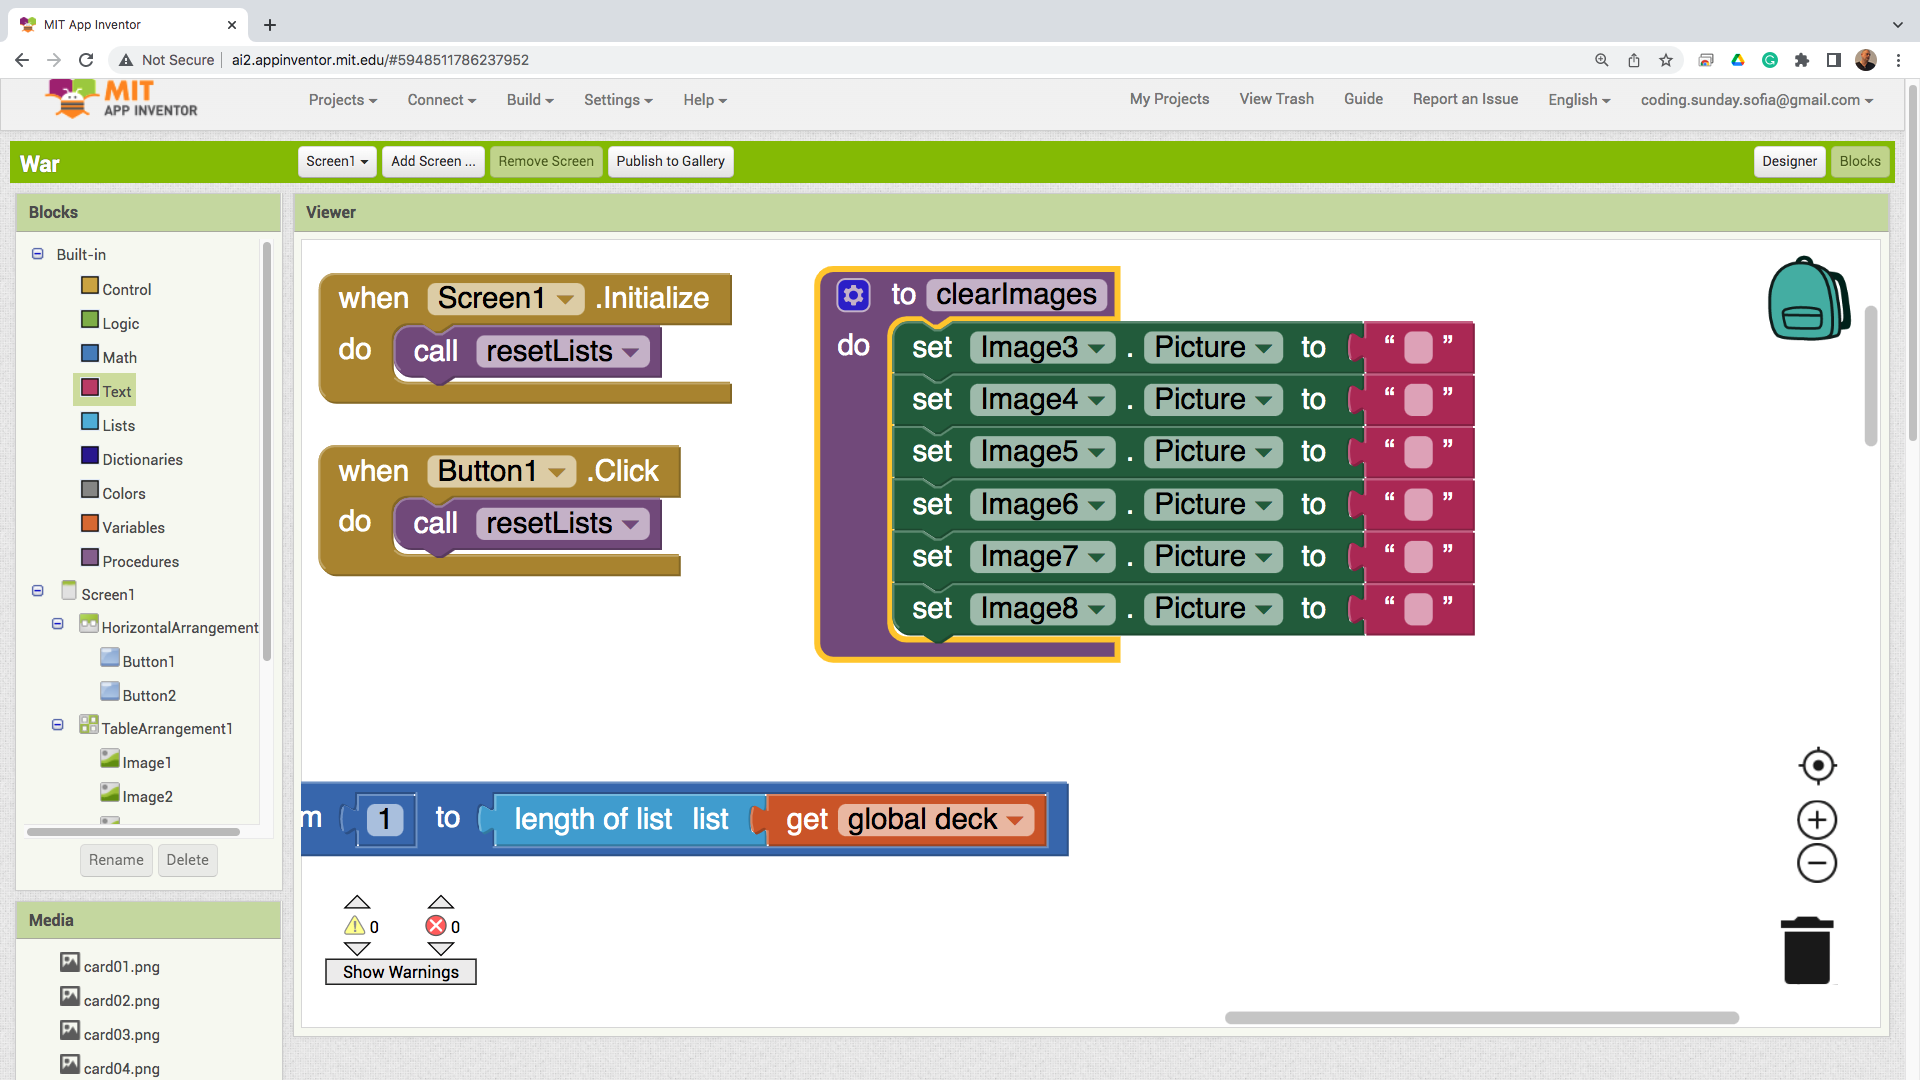
\includegraphics[width=1.0\linewidth,height=0.5\linewidth]{fig100016.png}
  \caption{Процедура за изчистване на картинките}
\label{fig100016}
\end{figure}

Натискането на втория бутон придвижва играта стъпка напред. Първата му задача е да почисти визуализираните карти от предходния ход (Фиг. \ref{fig100017}). След което следва каскада от възможни ситуации.

\begin{figure}[H]
  \centering
  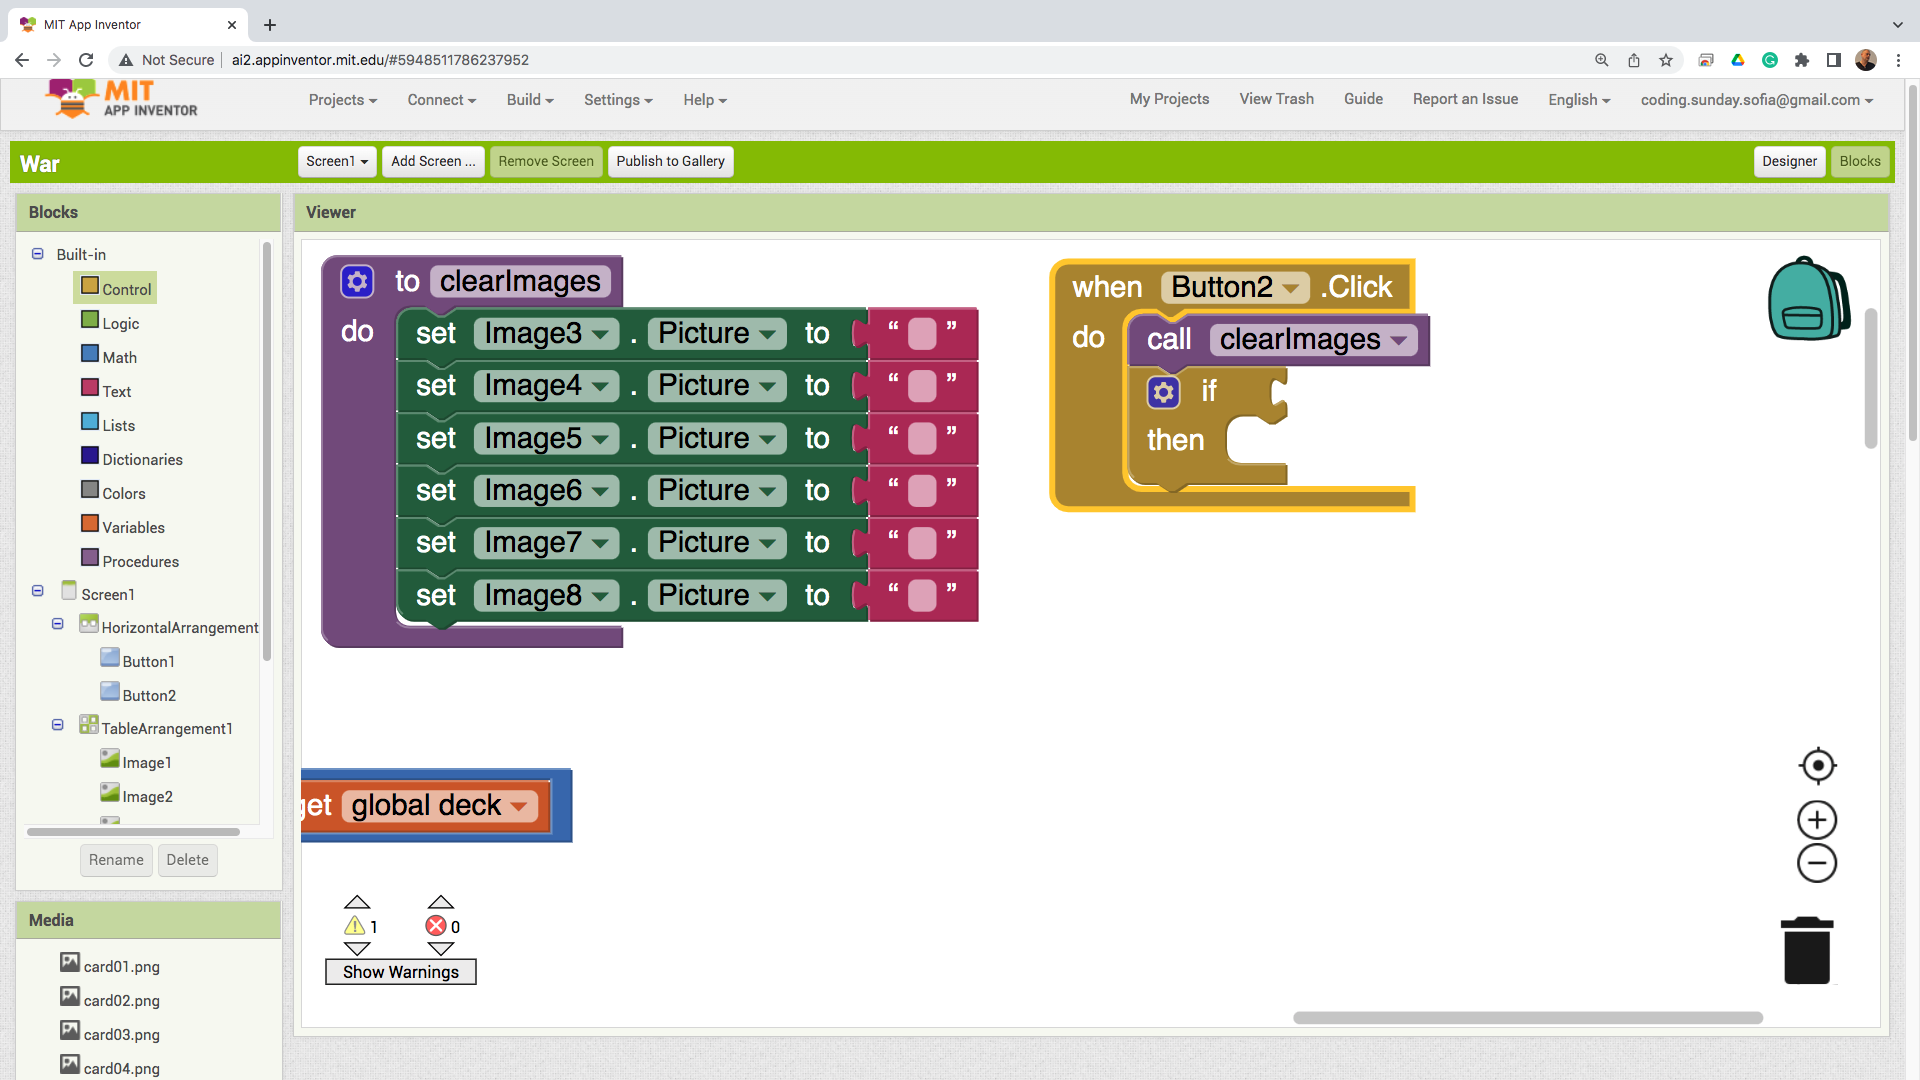
\includegraphics[width=1.0\linewidth,height=0.5\linewidth]{fig100017.png}
  \caption{Прихващане на събитие за следваща стъпка в играта}
\label{fig100017}
\end{figure}

Първите две ситуации на игралното табло са когато единият играч има карти в ръката си, другият няма и на масата също няма карти (Фиг. \ref{fig100018}). В тази ситуация, играчът който има карти в ръката си е победител.

\begin{figure}[H]
  \centering
  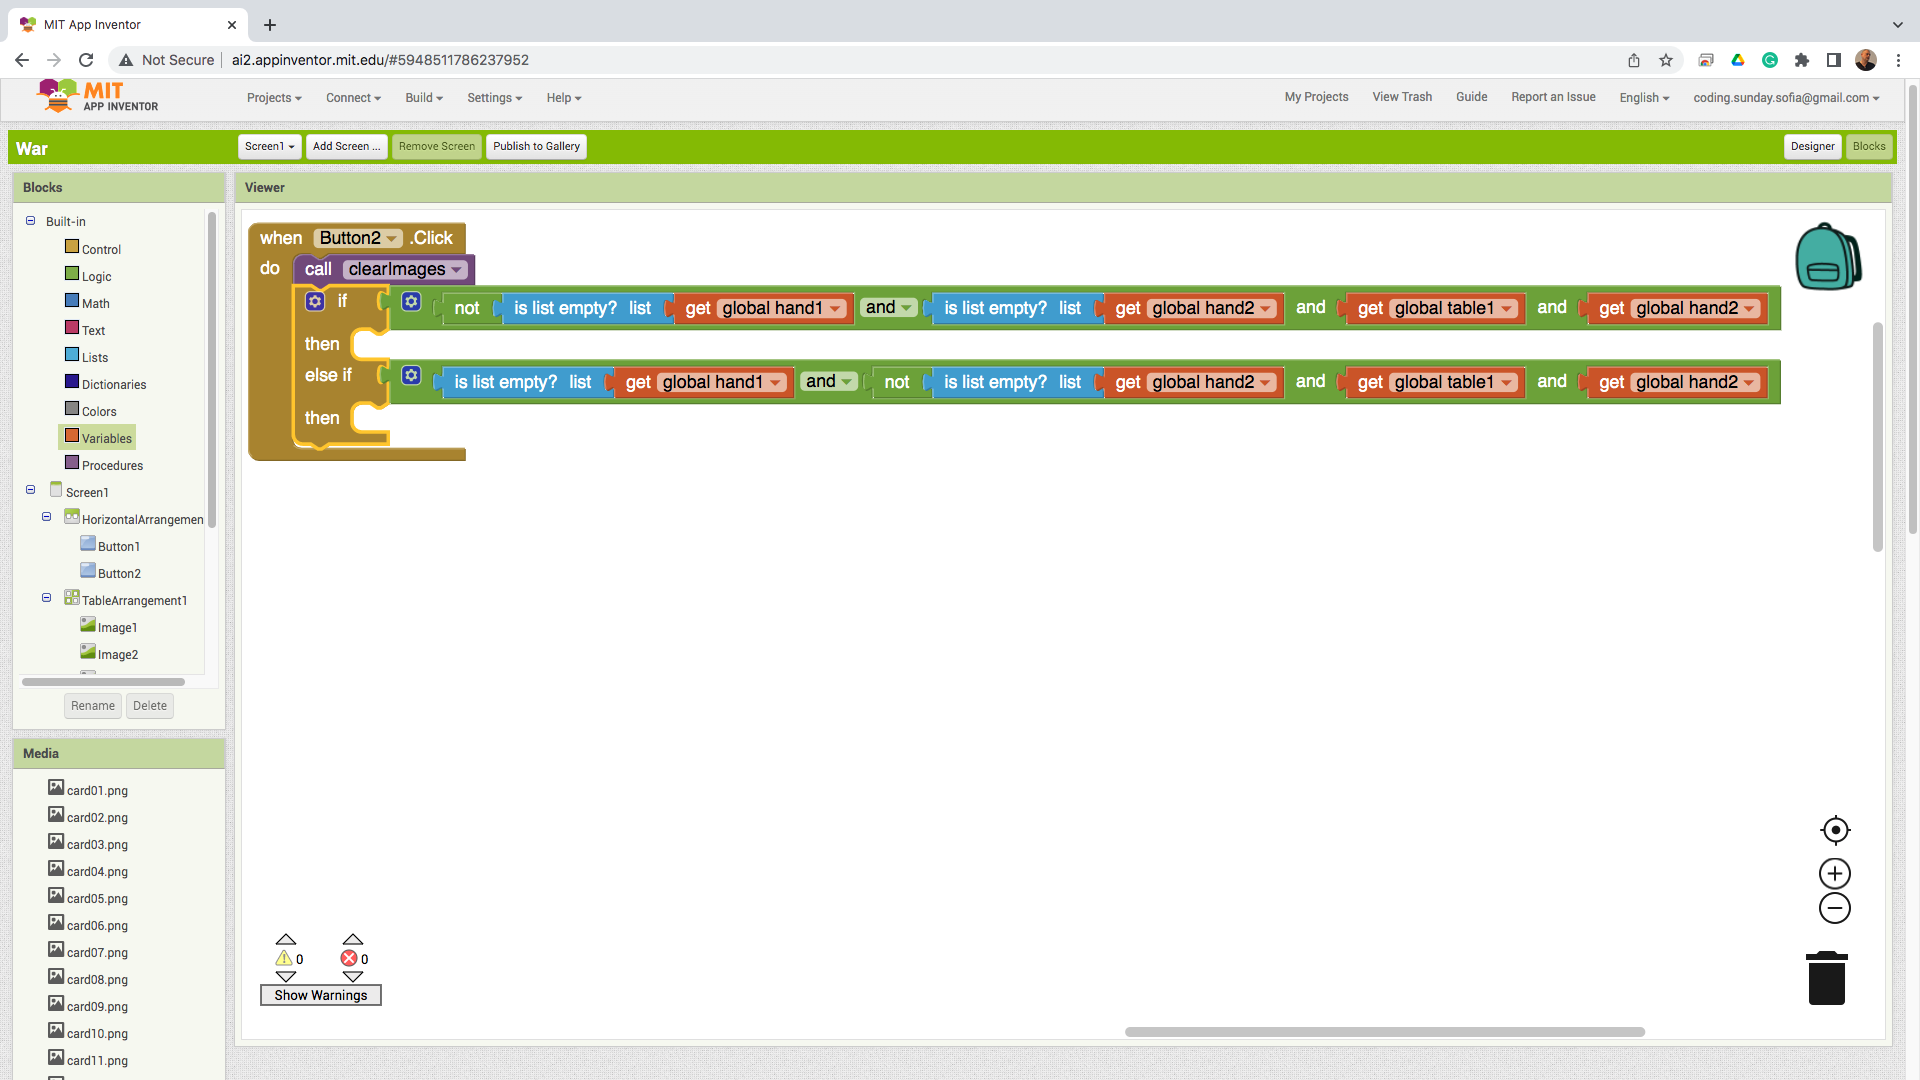
\includegraphics[width=1.0\linewidth,height=0.5\linewidth]{fig100018.png}
  \caption{Ситуации с вече определен победител}
\label{fig100018}
\end{figure}

Вторите две ситуации (Фиг. \ref{fig100019}) са когато на масата няма карти, тоест трябва да се извадят от тестетата и когато на масата има карти и трябва да се определи кой играч печели рунда.

\begin{figure}[H]
  \centering
  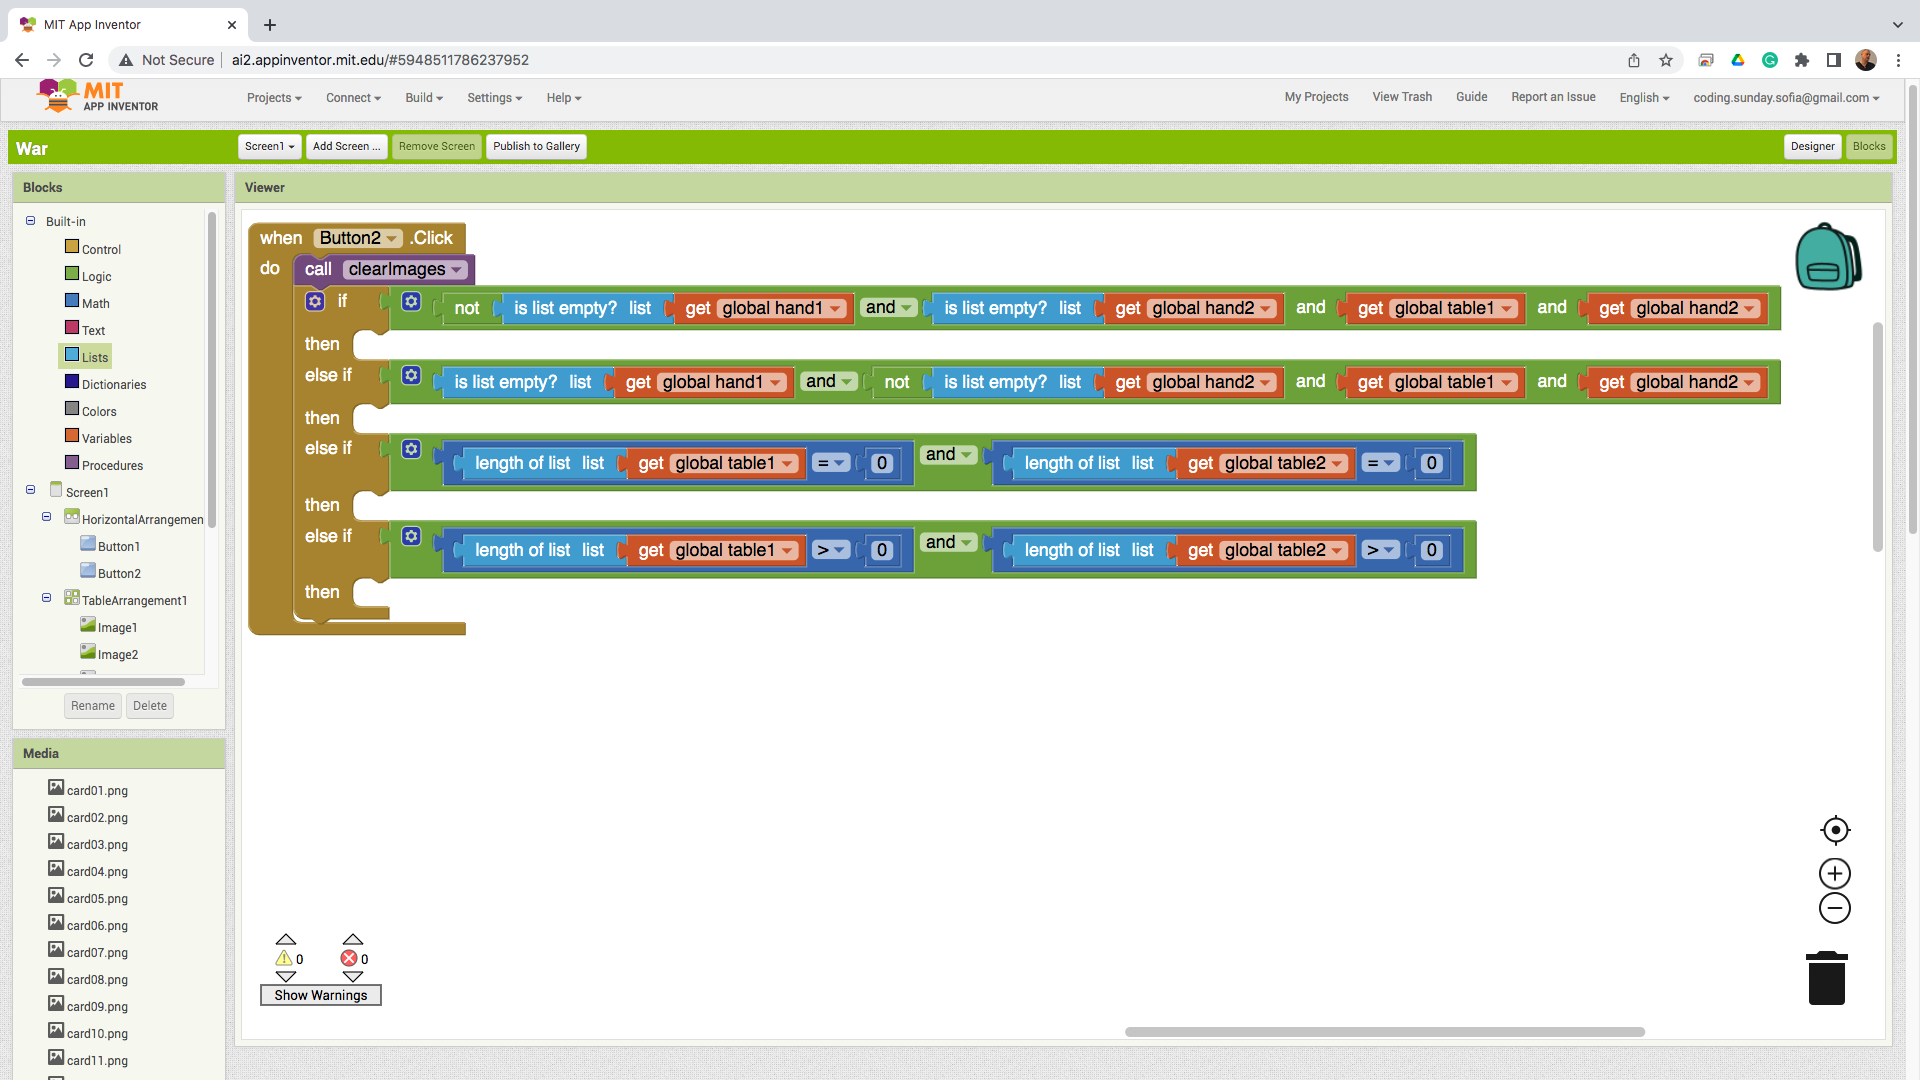
\includegraphics[width=1.0\linewidth,height=0.5\linewidth]{fig100019.png}
  \caption{Ситуации според наличието на карти на масата}
\label{fig100019}
\end{figure}

За първите две състояния единствено се обявява в съобщение кой е победителят. За вторите две състояние се обособяват помощни функции. Веднага след възможните състояние следва помощна функция за обновяване на визуалното пространство (Фиг. \ref{fig100020}).

\begin{figure}[H]
  \centering
  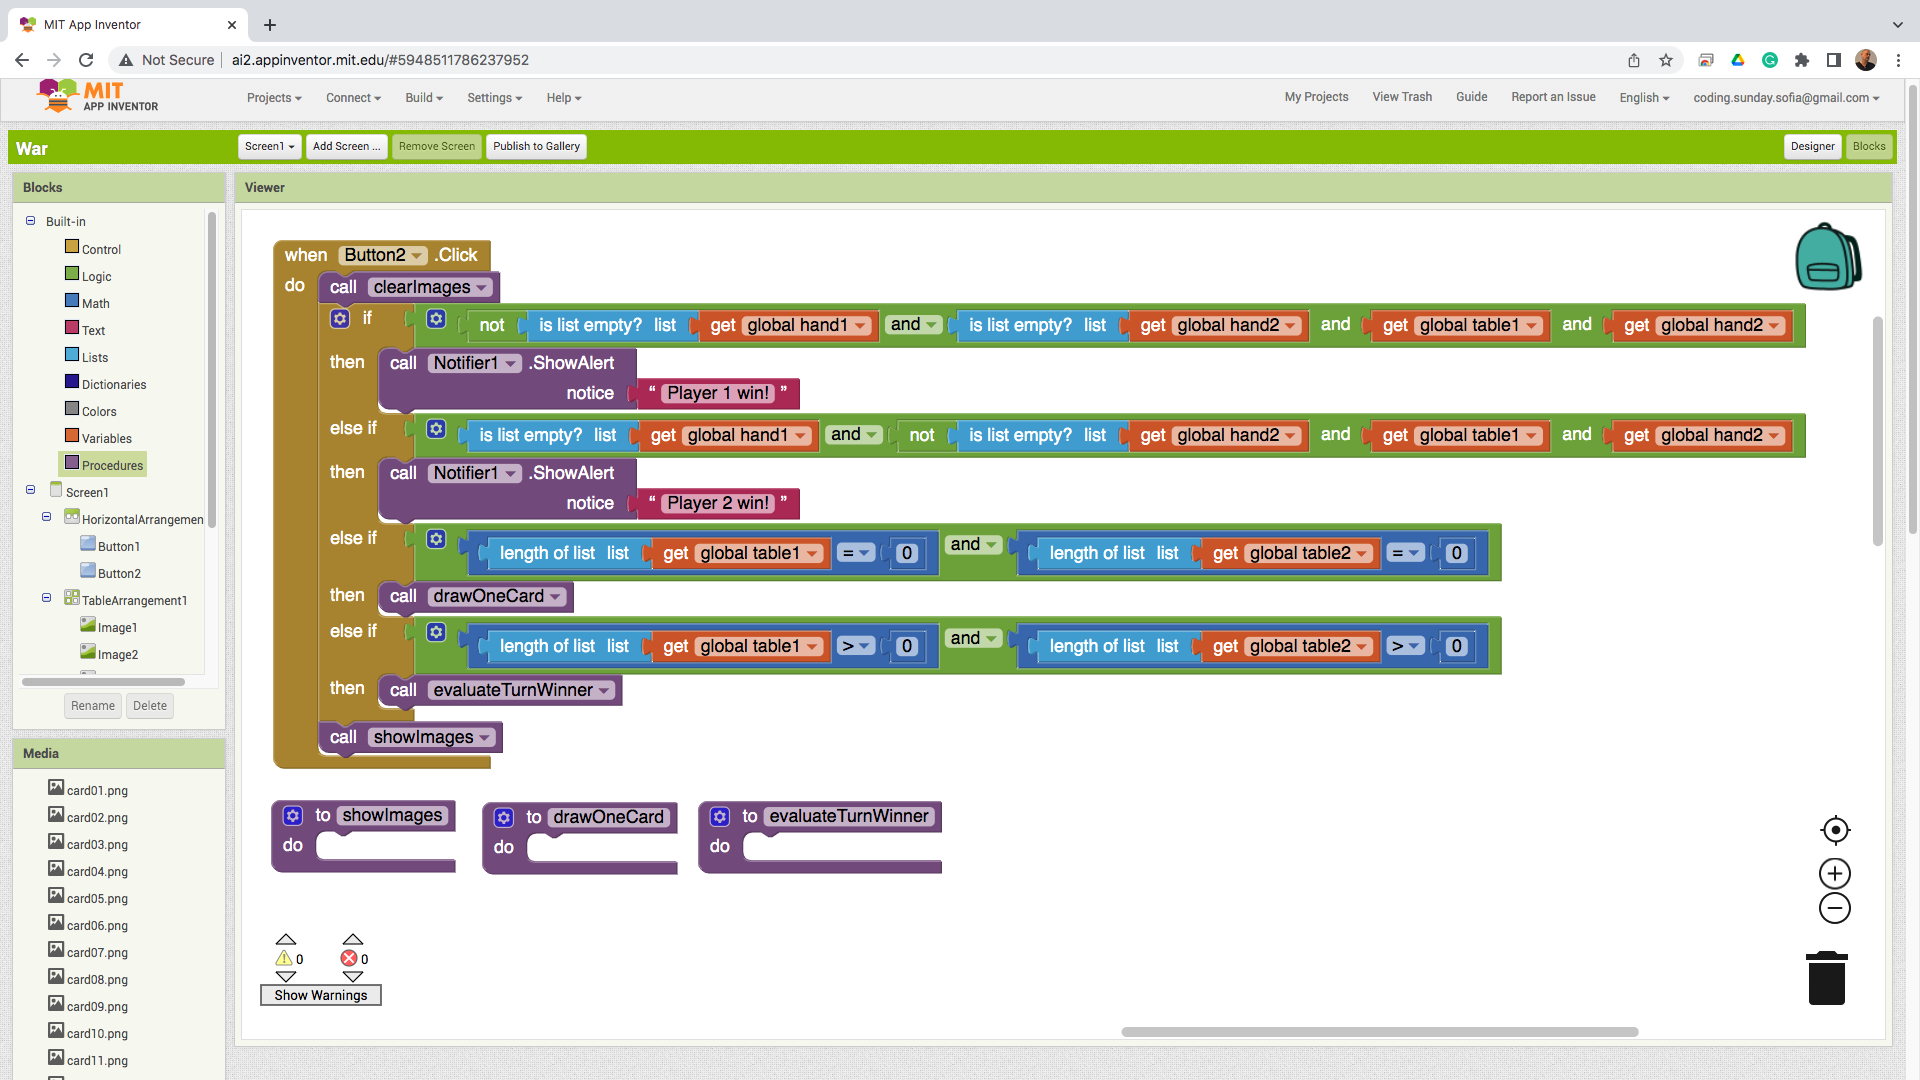
\includegraphics[width=1.0\linewidth,height=0.5\linewidth]{fig100020.png}
  \caption{Помощни функции за отработване на различните ситуации}
\label{fig100020}
\end{figure}

Помощната функция за визуализация на картите върху масата, в най-сложния случай, показва не повече от по три карти за играч, тоест общо шест. Когато няма състояние на война се визуализира една карата, когато има състояние на война се визуализират трите карти от последната война (войните може да са няколко поредни). Визуализацията се случва в два последователни цикъла (Фиг. \ref{fig100021}).

\begin{figure}[H]
  \centering
  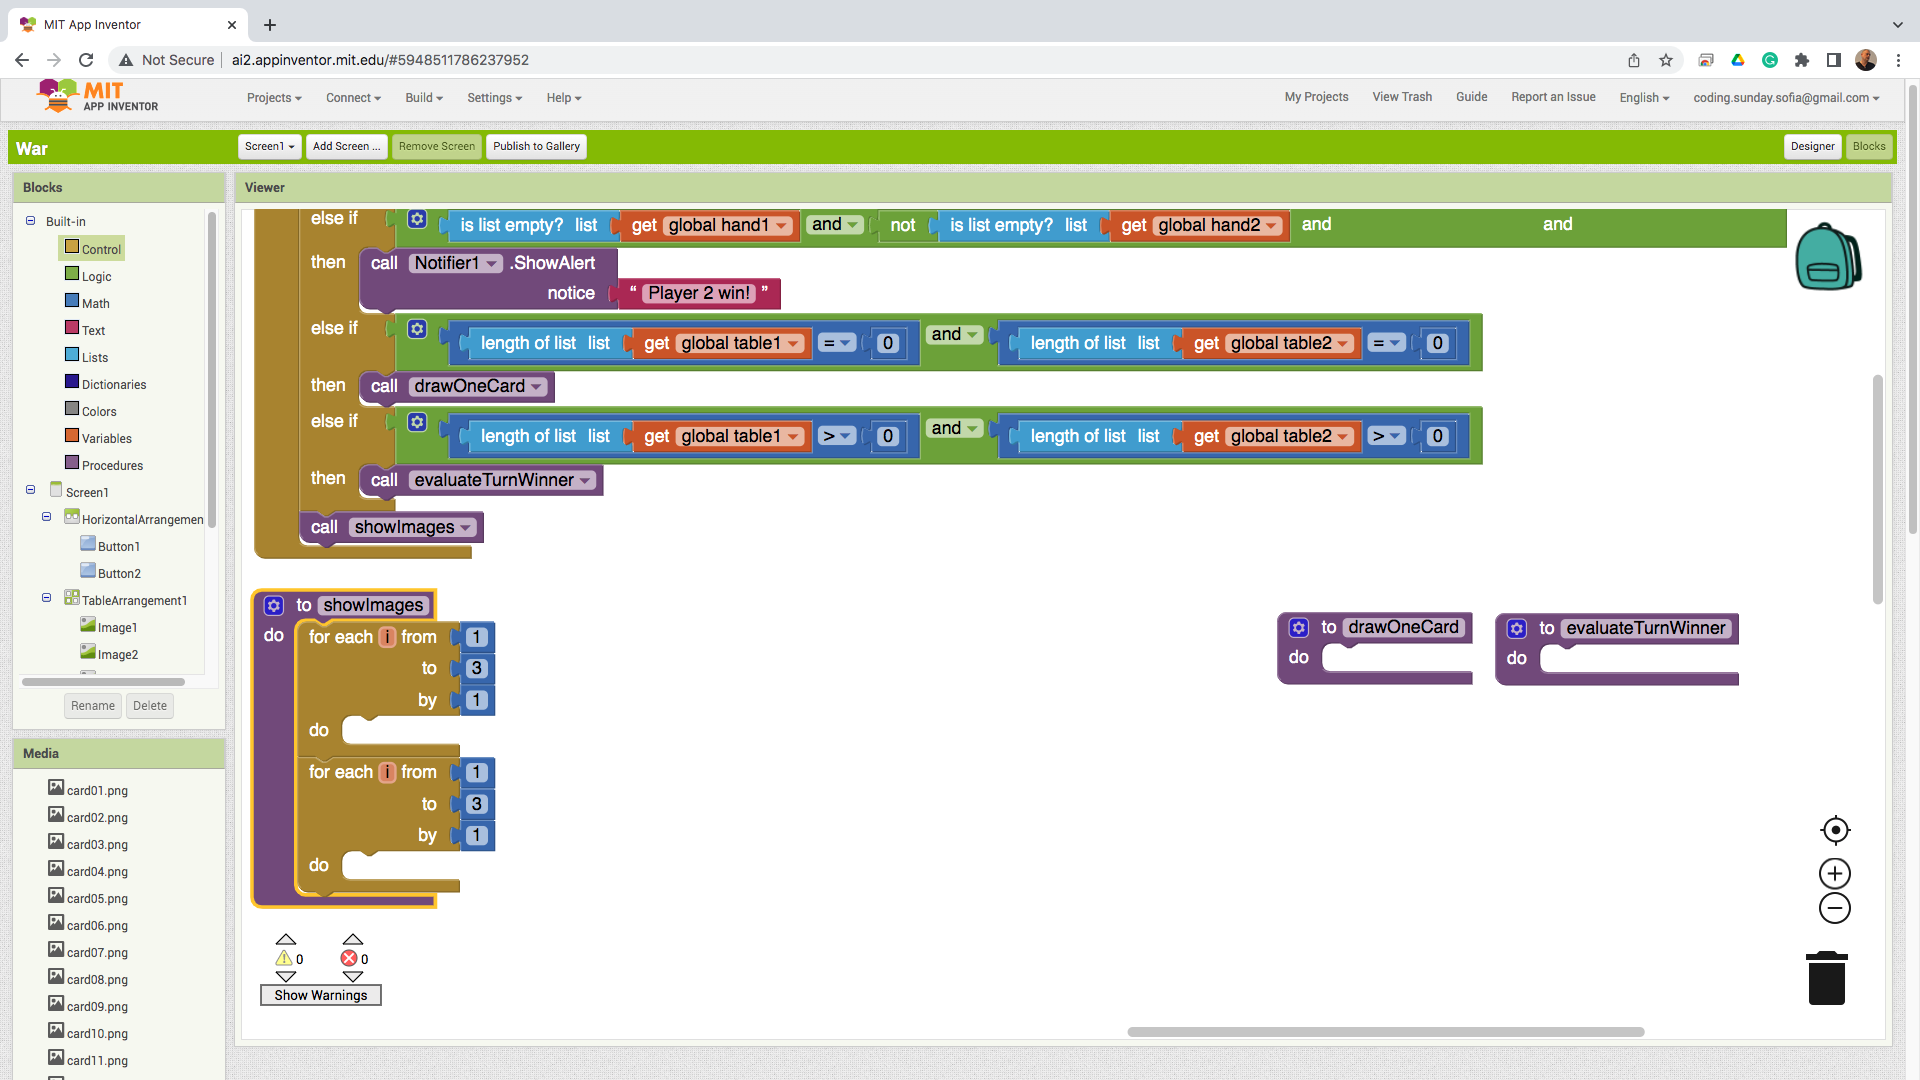
\includegraphics[width=1.0\linewidth,height=0.5\linewidth]{fig100021.png}
  \caption{Цикли за визуализация на картите на масата}
\label{fig100021}
\end{figure}

Ако в списъците за карти на масата няма достатъчно елементи, то цикълът за визуализация трябва да бъде прекъснат (Фиг. \ref{fig100022}). Пример за такава ситуация е когато се появи състояние на война, но единия играч са му останали само две последни карти.

\begin{figure}[H]
  \centering
  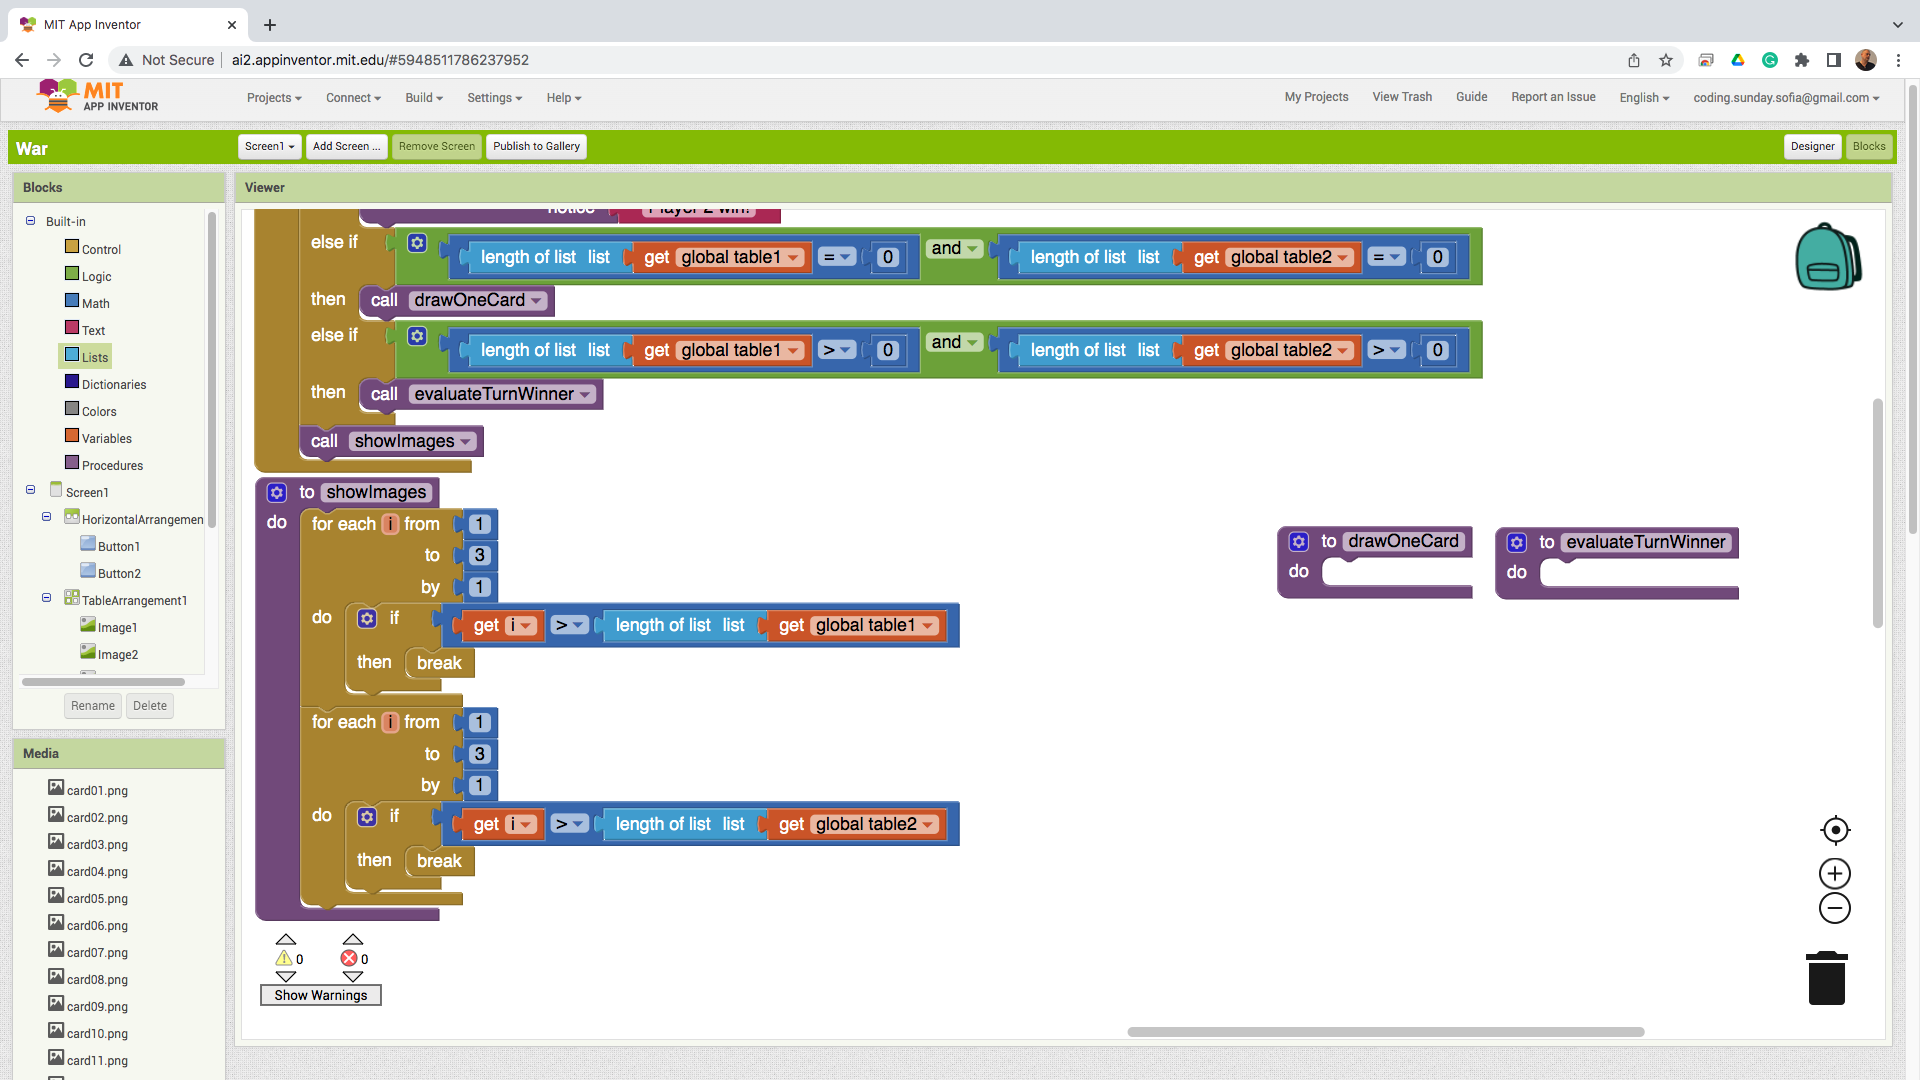
\includegraphics[width=1.0\linewidth,height=0.5\linewidth]{fig100022.png}
  \caption{Спиране на визуализацията при недостиг на карти}
\label{fig100022}
\end{figure}

При наличие на достатъчно карти на масата, в компонента за визуализация на картинки се показва това изображение от списъка с изображенията, което е посочено като индекс в списъка с карти на масата (Фиг. \ref{fig100023}).

\begin{figure}[H]
  \centering
  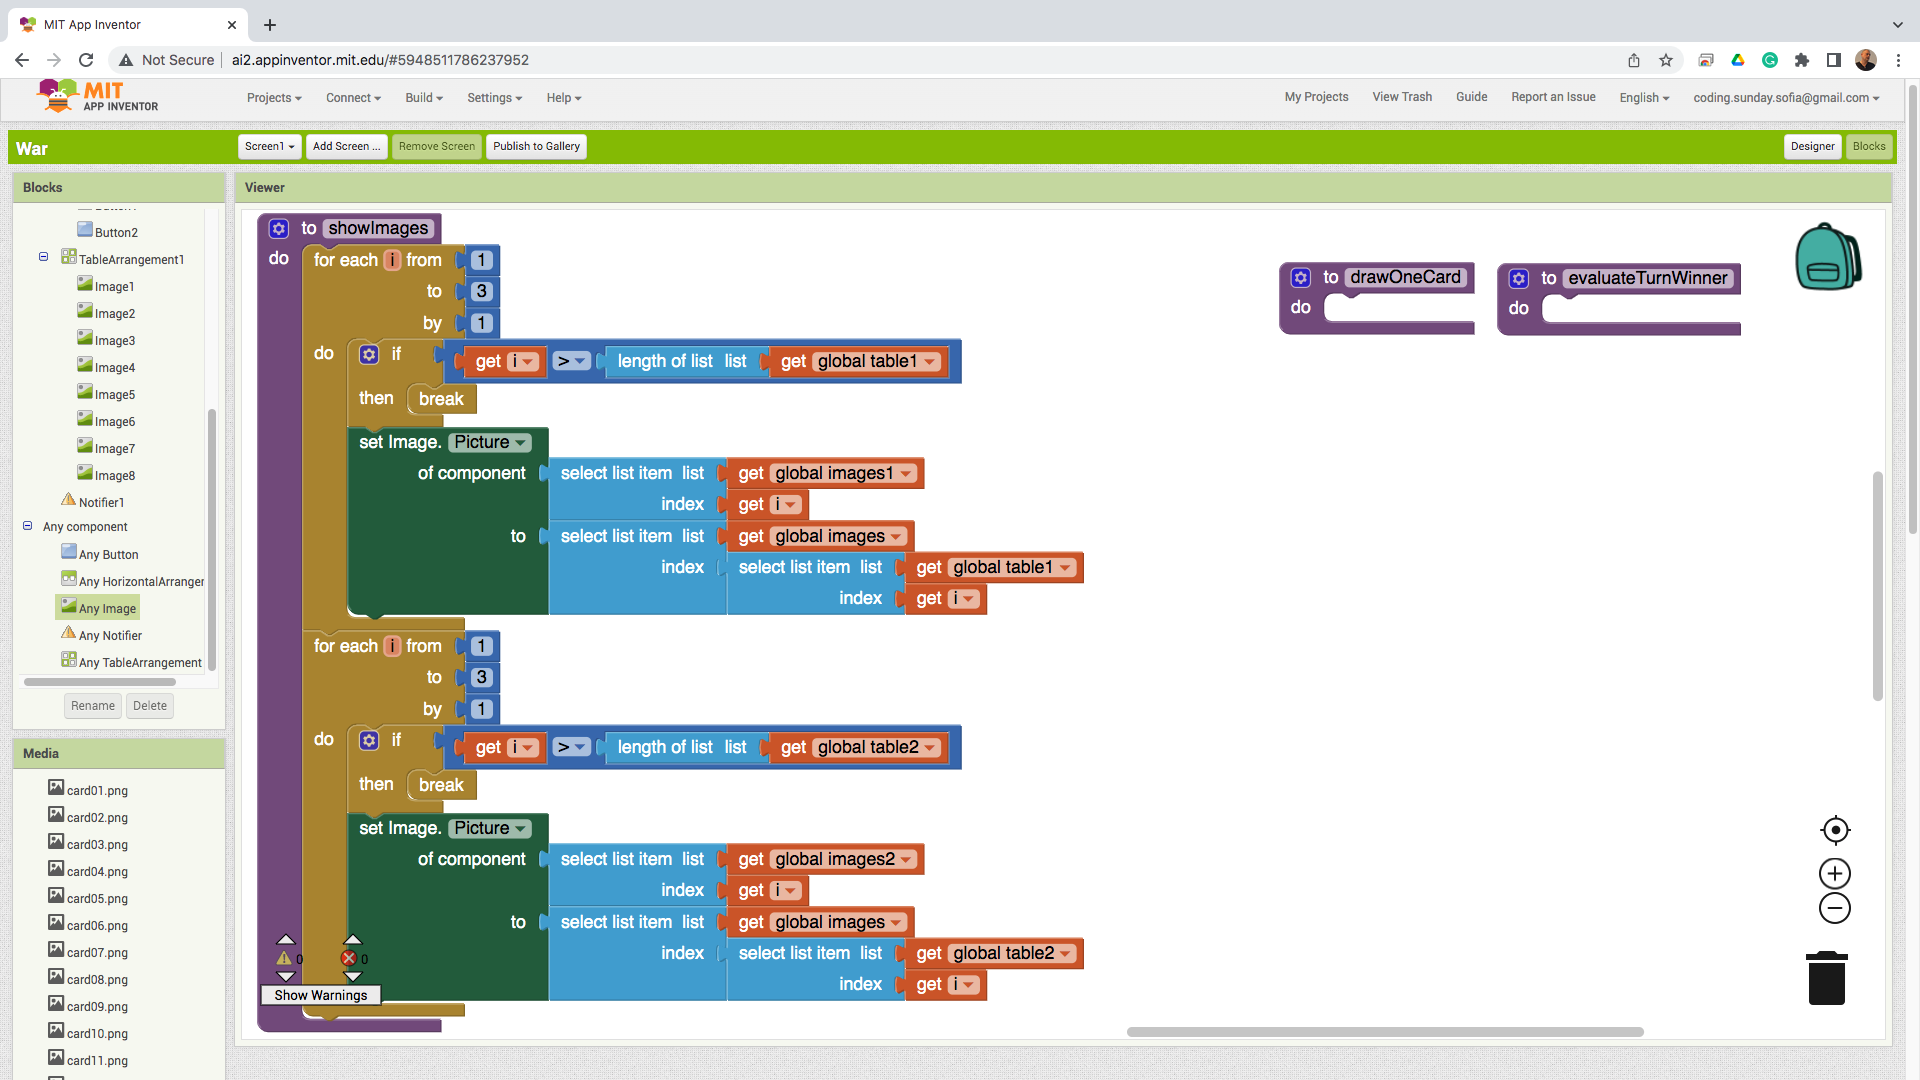
\includegraphics[width=1.0\linewidth,height=0.5\linewidth]{fig100023.png}
  \caption{Определяне на кои изображения да бъдат показани}
\label{fig100023}
\end{figure}

За да изтегли по една карта, всеки играч трябва да вземе картата от ръката си, на първо място, и да я постави на първо място в реда с карти на масата (Фиг. \ref{fig100024}). Картата постъпва в списъка за масата и напуска списъка за ръката.

\begin{figure}[H]
  \centering
  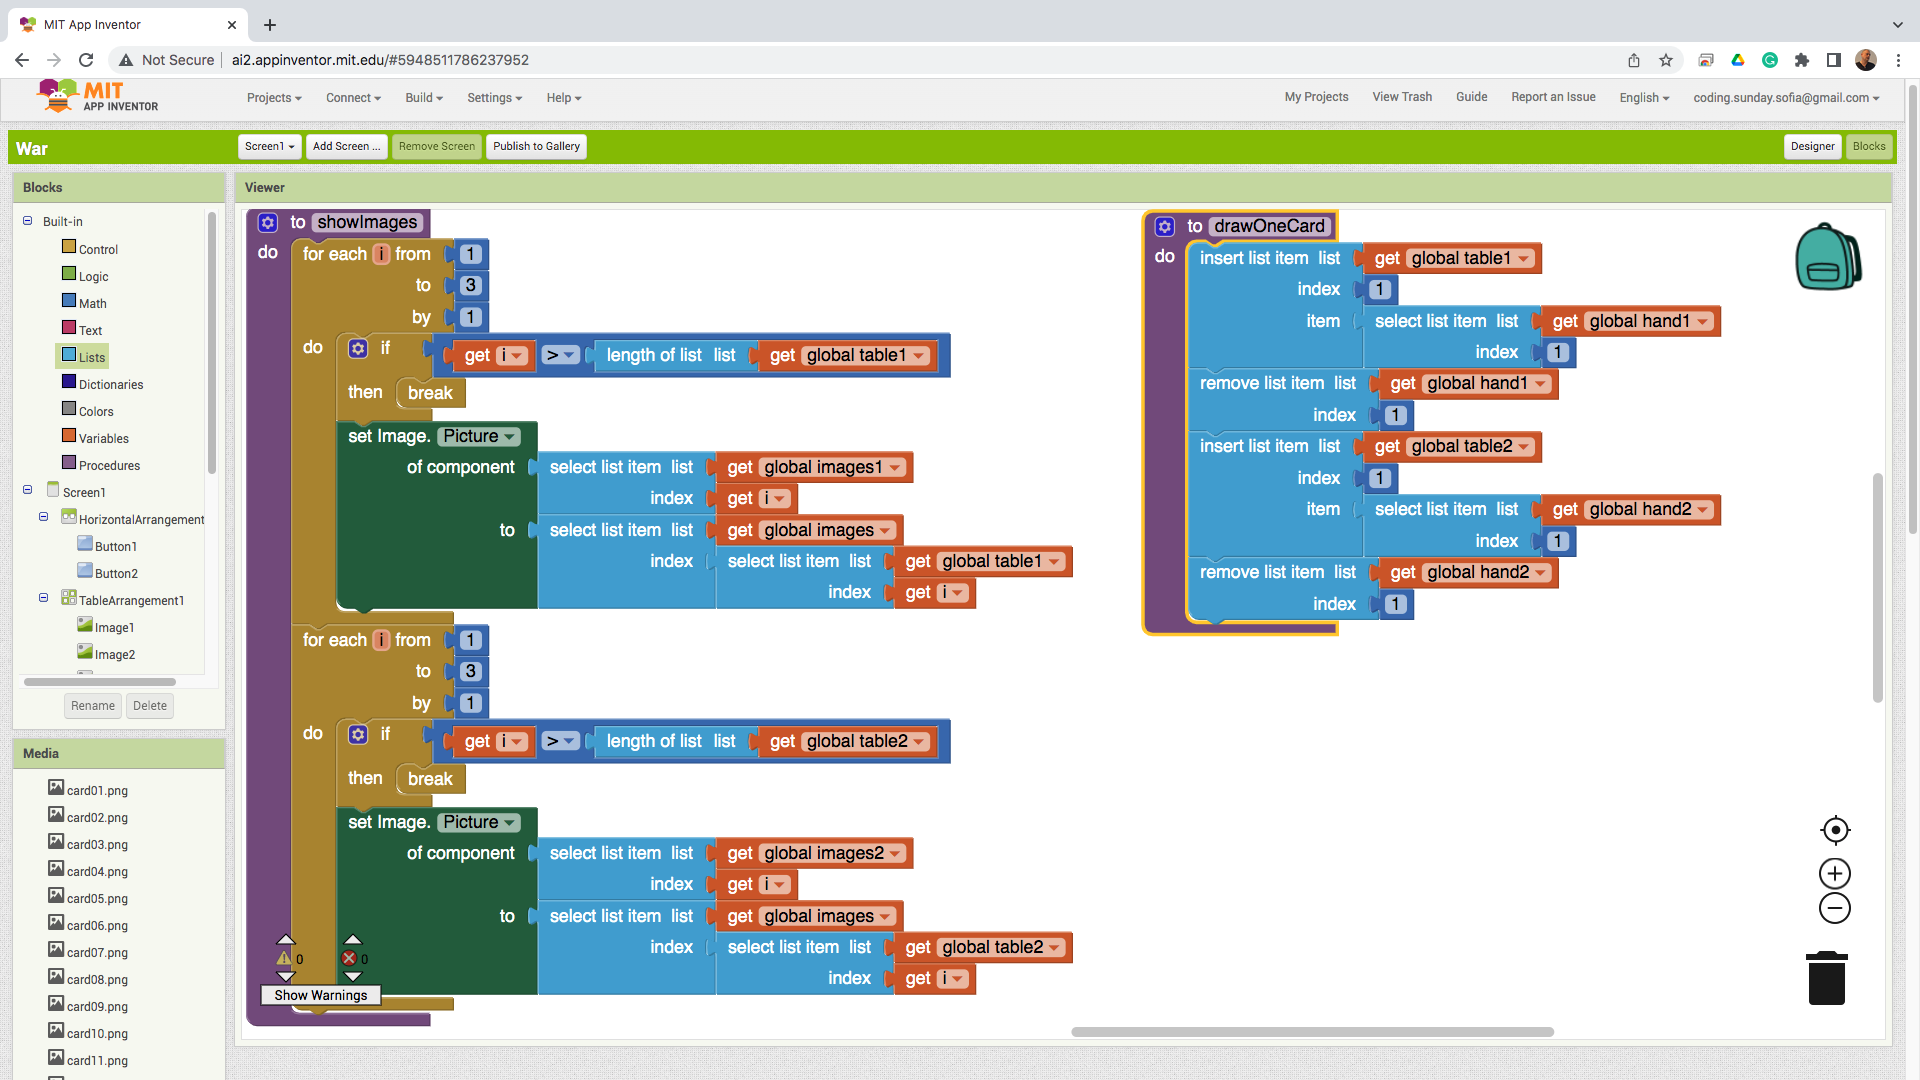
\includegraphics[width=1.0\linewidth,height=0.5\linewidth]{fig100024.png}
  \caption{Изтегляне на по една карта}
\label{fig100024}
\end{figure}

Когато има карти на масата са възможни три ситуации – ходът се печели от първия играч, ходът се печели от втория играчи и играчите са на равно, което води до състояние на война (Фиг. \ref{fig100025}). Картите в основното тесте са така подредени, че формират подгрупи от по четири, спрямо силата, която имат. Поради тази причина, при целочислено делене надве, лесно може да се определи коя карта побеждава. Трябва да се извади единица, тъй като номерацията в основното тесте започва от едно и стига до 52, а целочисленото деление може да се приложи при номерация от 0 до 51. 

\begin{figure}[H]
  \centering
  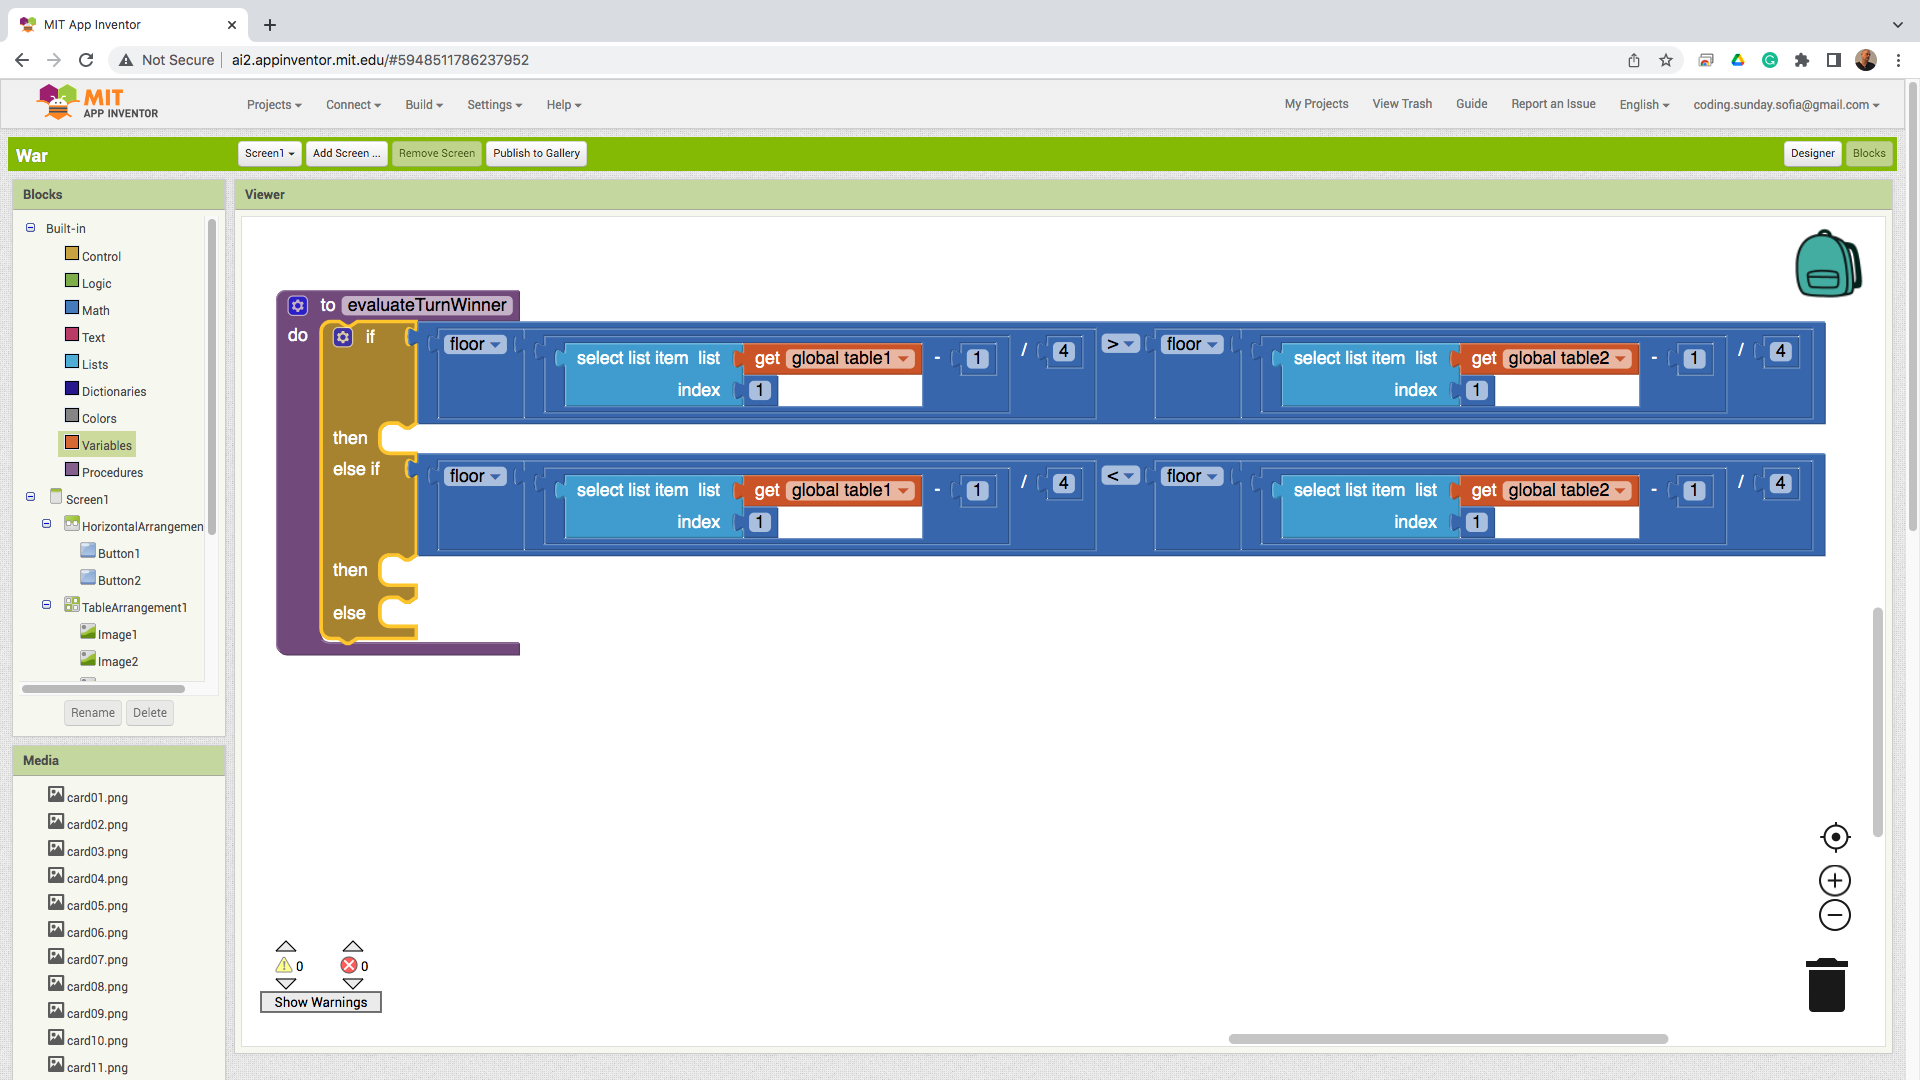
\includegraphics[width=1.0\linewidth,height=0.5\linewidth]{fig100025.png}
  \caption{Възможни ситуации при карти на масата}
\label{fig100025}
\end{figure}

Ако в текущия ход побеждава първият играч, то той прибира в ръката си своите карти от масата и картите от масата на втория играч. Ако в текущия ход побеждава вторият играч, то той прибира своите карти от масата и картите на противника от масата. Тези действия се извършват с допълване на списък с ръка и изпразване на списъците за масата (Фиг. \ref{fig100026}).

\begin{figure}[H]
  \centering
  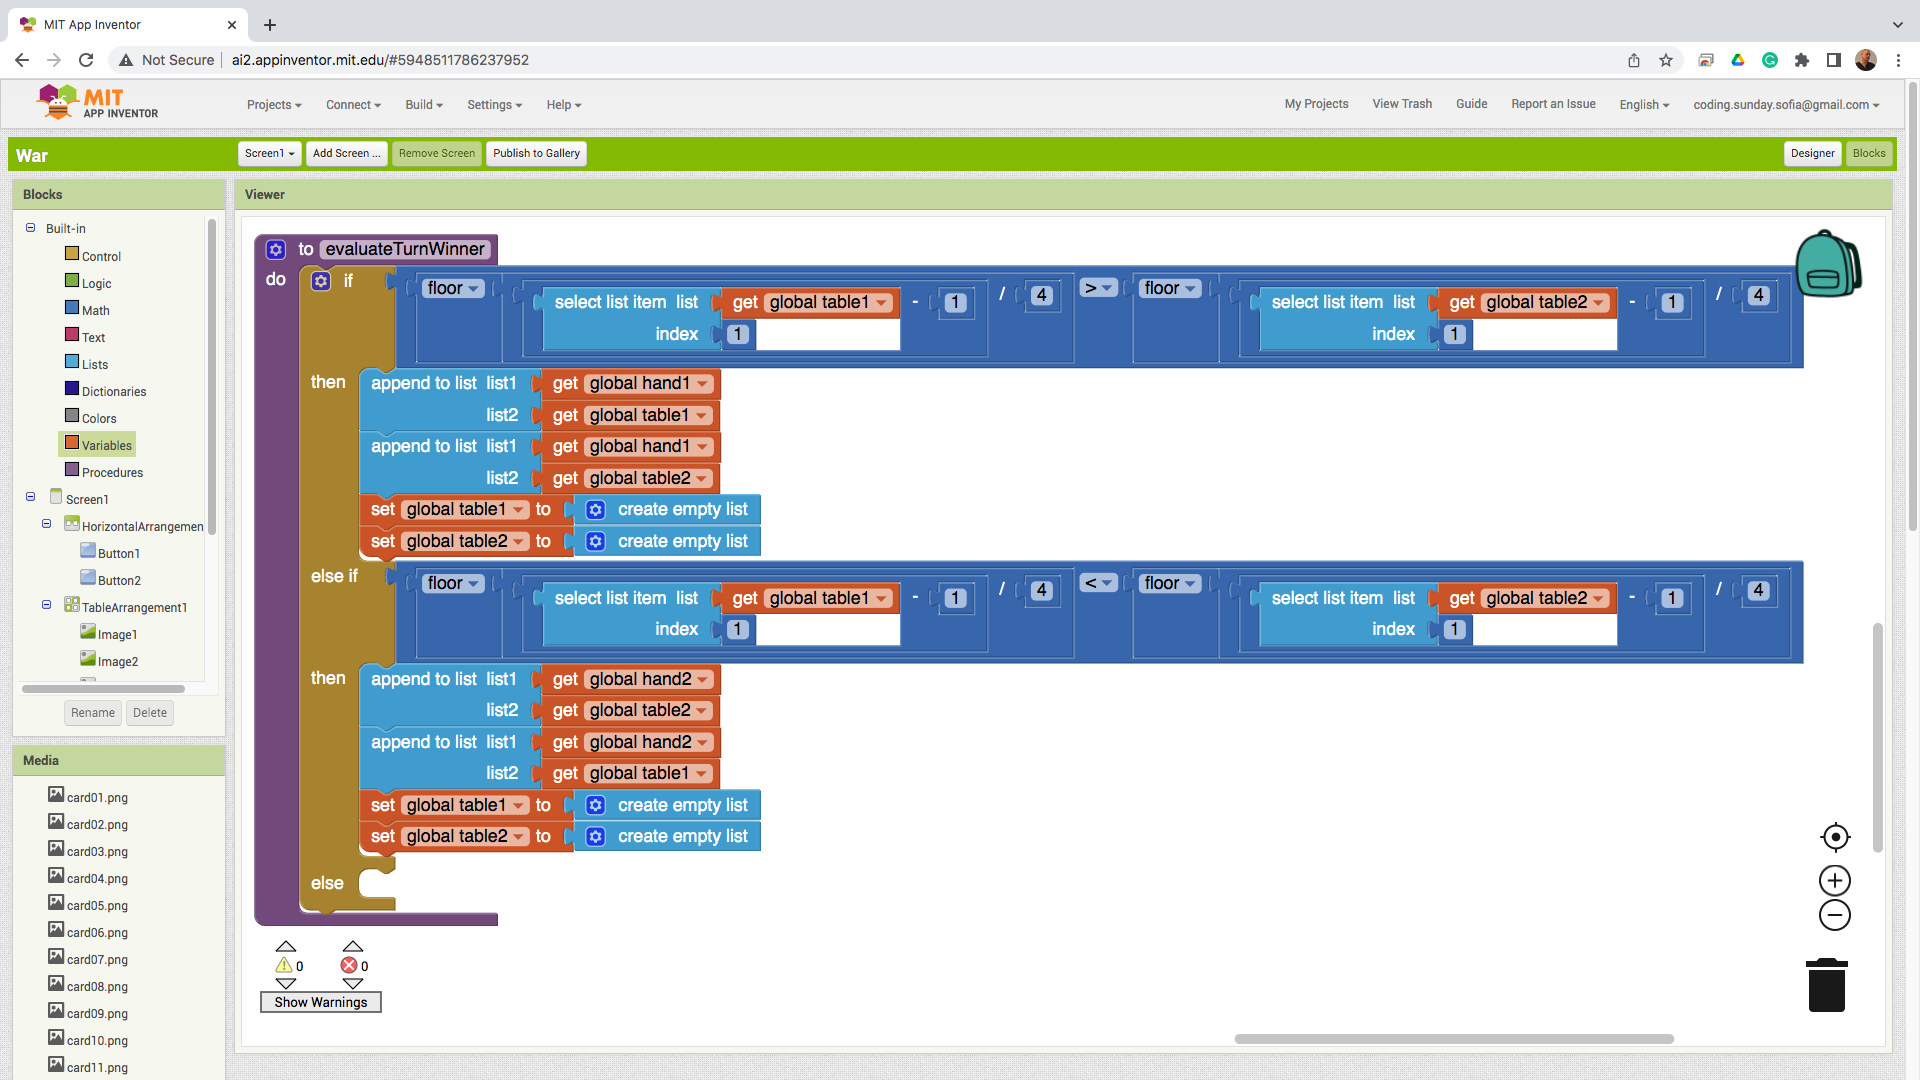
\includegraphics[width=1.0\linewidth,height=0.5\linewidth]{fig100026.png}
  \caption{Събиране на картите след победа в отделен ход на играта}
\label{fig100026}
\end{figure}

При състояние на война, всеки от играчите изважда по три карти, с които участва във войната. Това действие се случва в цикъл, въртящ се три пъти (Фиг. \ref{fig100027}).

\begin{figure}[H]
  \centering
  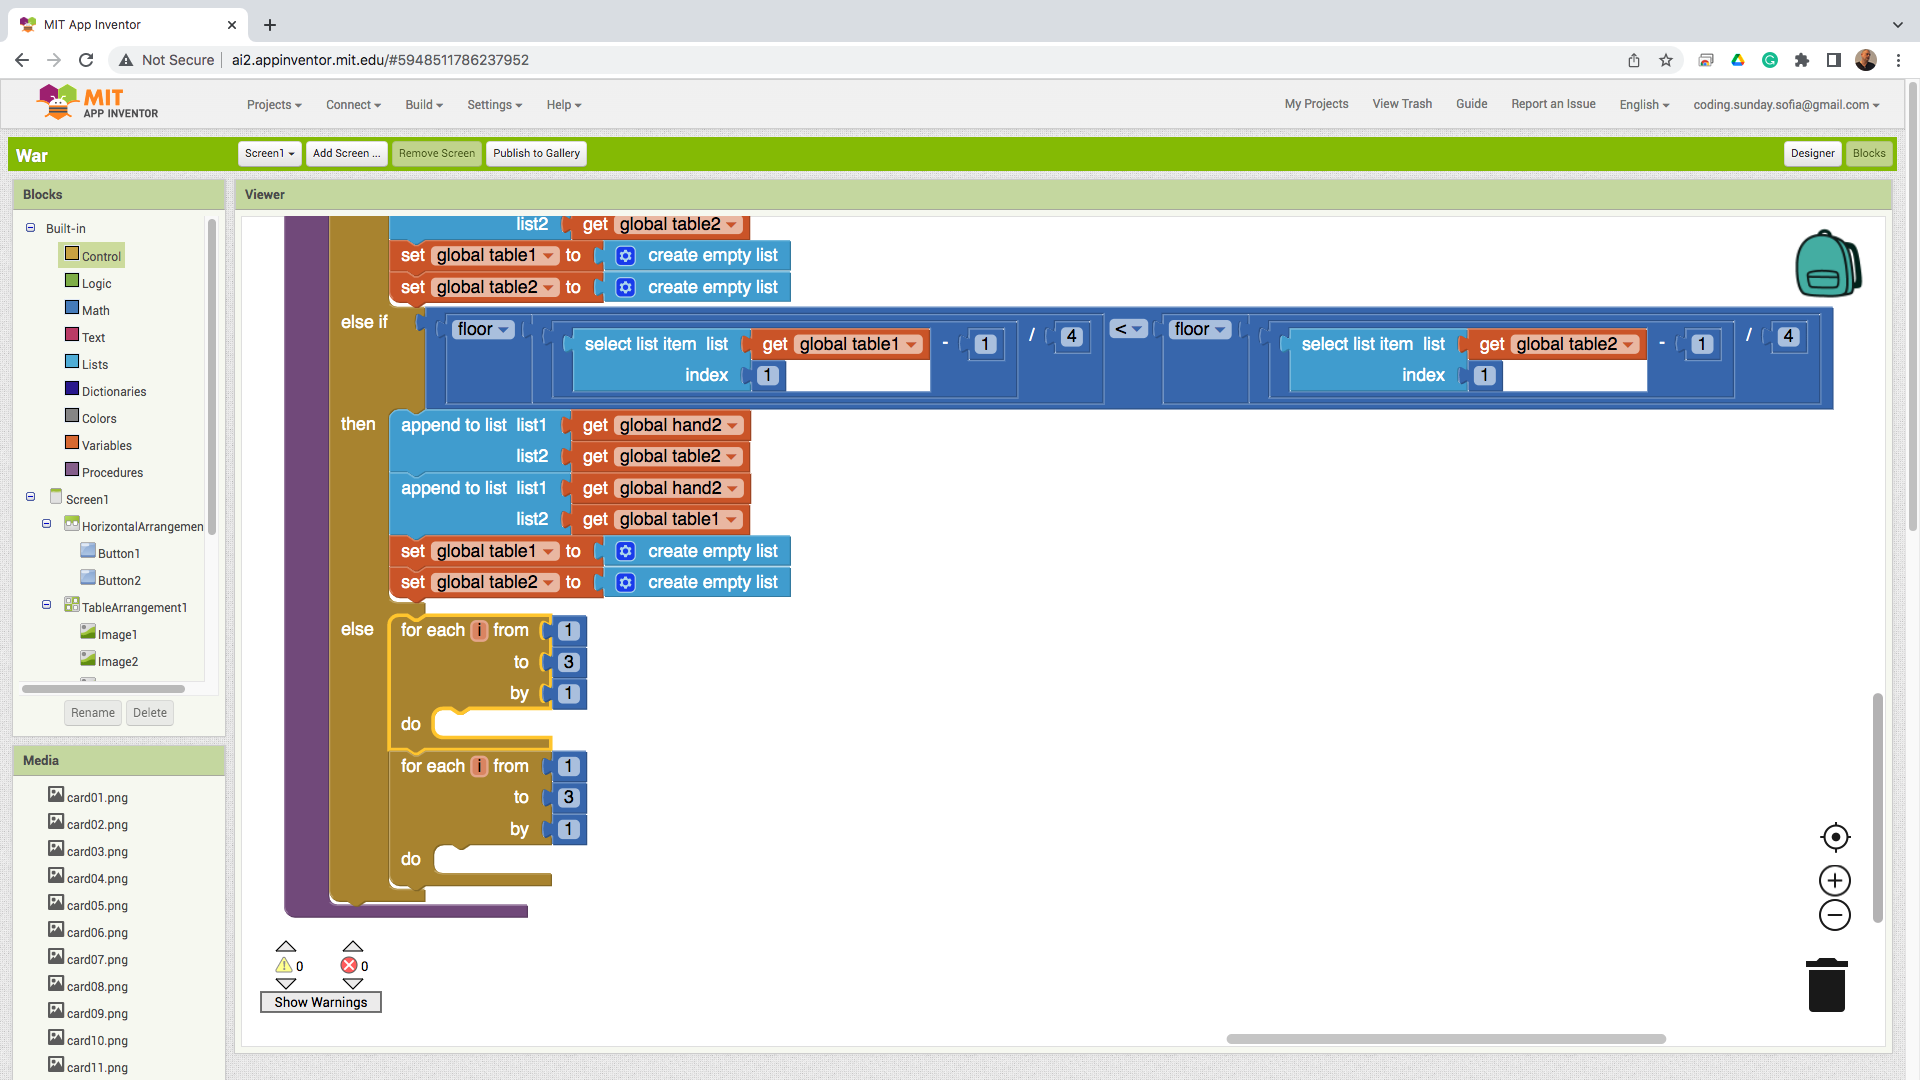
\includegraphics[width=1.0\linewidth,height=0.5\linewidth]{fig100027.png}
  \caption{Цикъл за показване на карти при война}
\label{fig100027}
\end{figure}

В процеса по теглене на карти за войната е възможно някой от играчите да остане без карти и да не може да тегли, тогава цикълът за теглене трябва да бъде спрян (Фиг. \ref{fig100028}).

\begin{figure}[H]
  \centering
  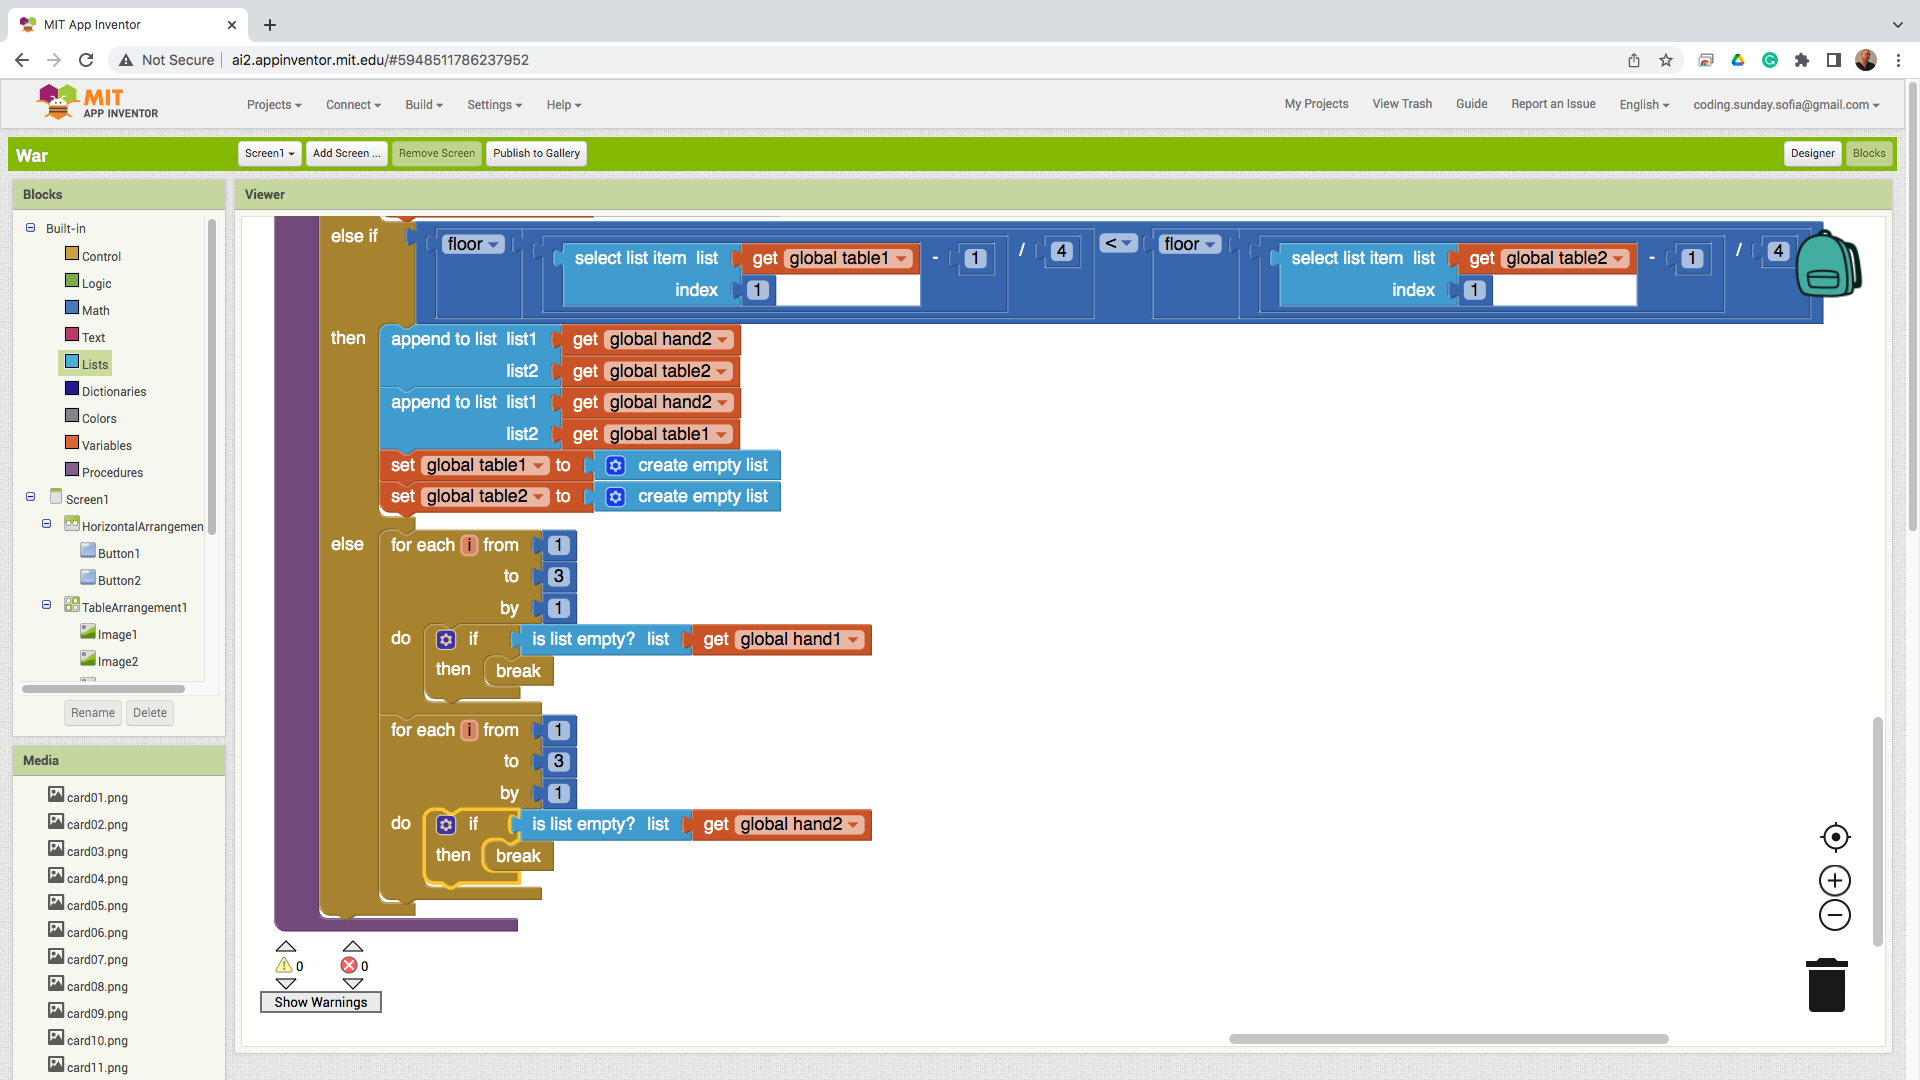
\includegraphics[width=1.0\linewidth,height=0.5\linewidth]{fig100028.png}
  \caption{Спиране на тегленето при изчерпване на картите}
\label{fig100028}
\end{figure}

Изваждането на карта и поставянето й на масата е случва по абсолютно идентичен начин, както е в процедурата по изваждане на една карта, но се случва три път (Фиг. \ref{fig100029}).

\begin{figure}[H]
  \centering
  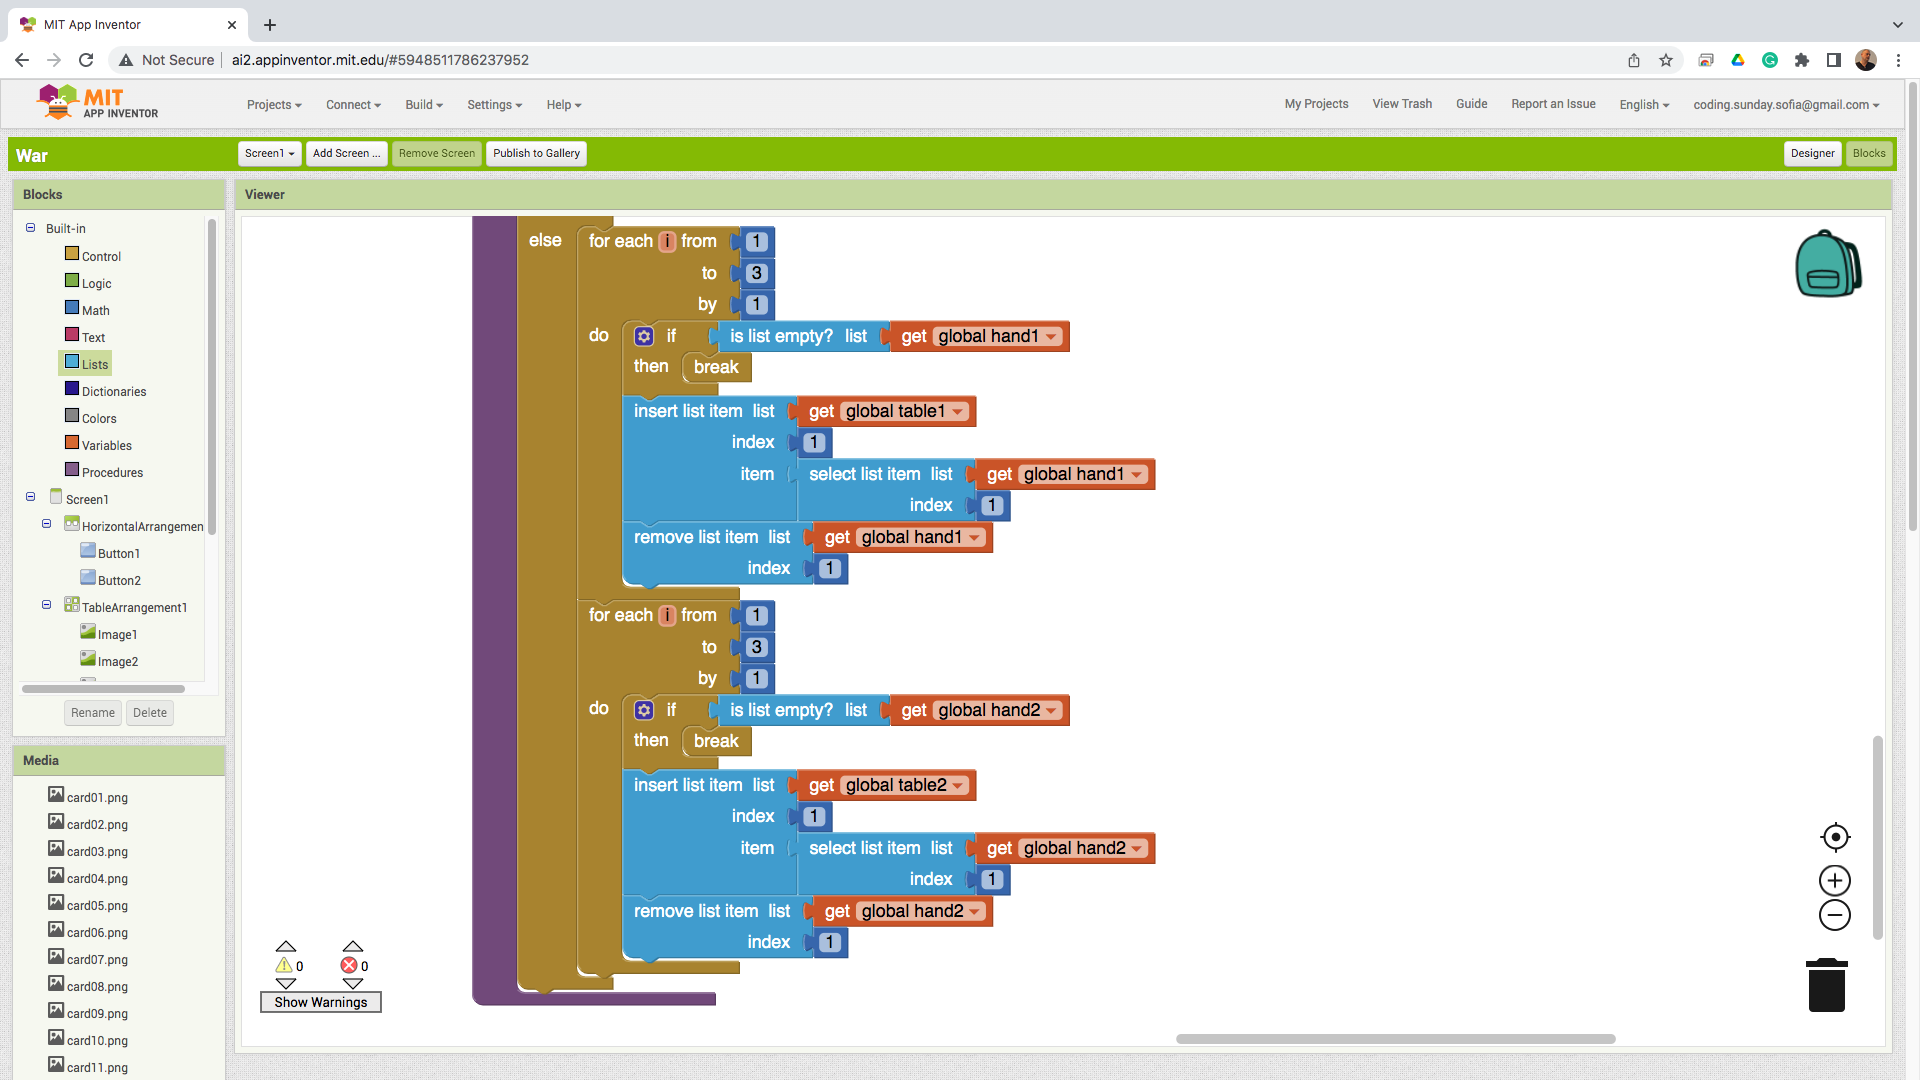
\includegraphics[width=1.0\linewidth,height=0.5\linewidth]{fig100029.png}
  \caption{Изваждане на по три карти на масата}
\label{fig100029}
\end{figure}

\section{Публикуване на проекта}

Играта се прави публично достъпна, чрез публикуването й в зоната „галерия“ (Фиг. \ref{fig100030}).

\begin{figure}[H]
  \centering
  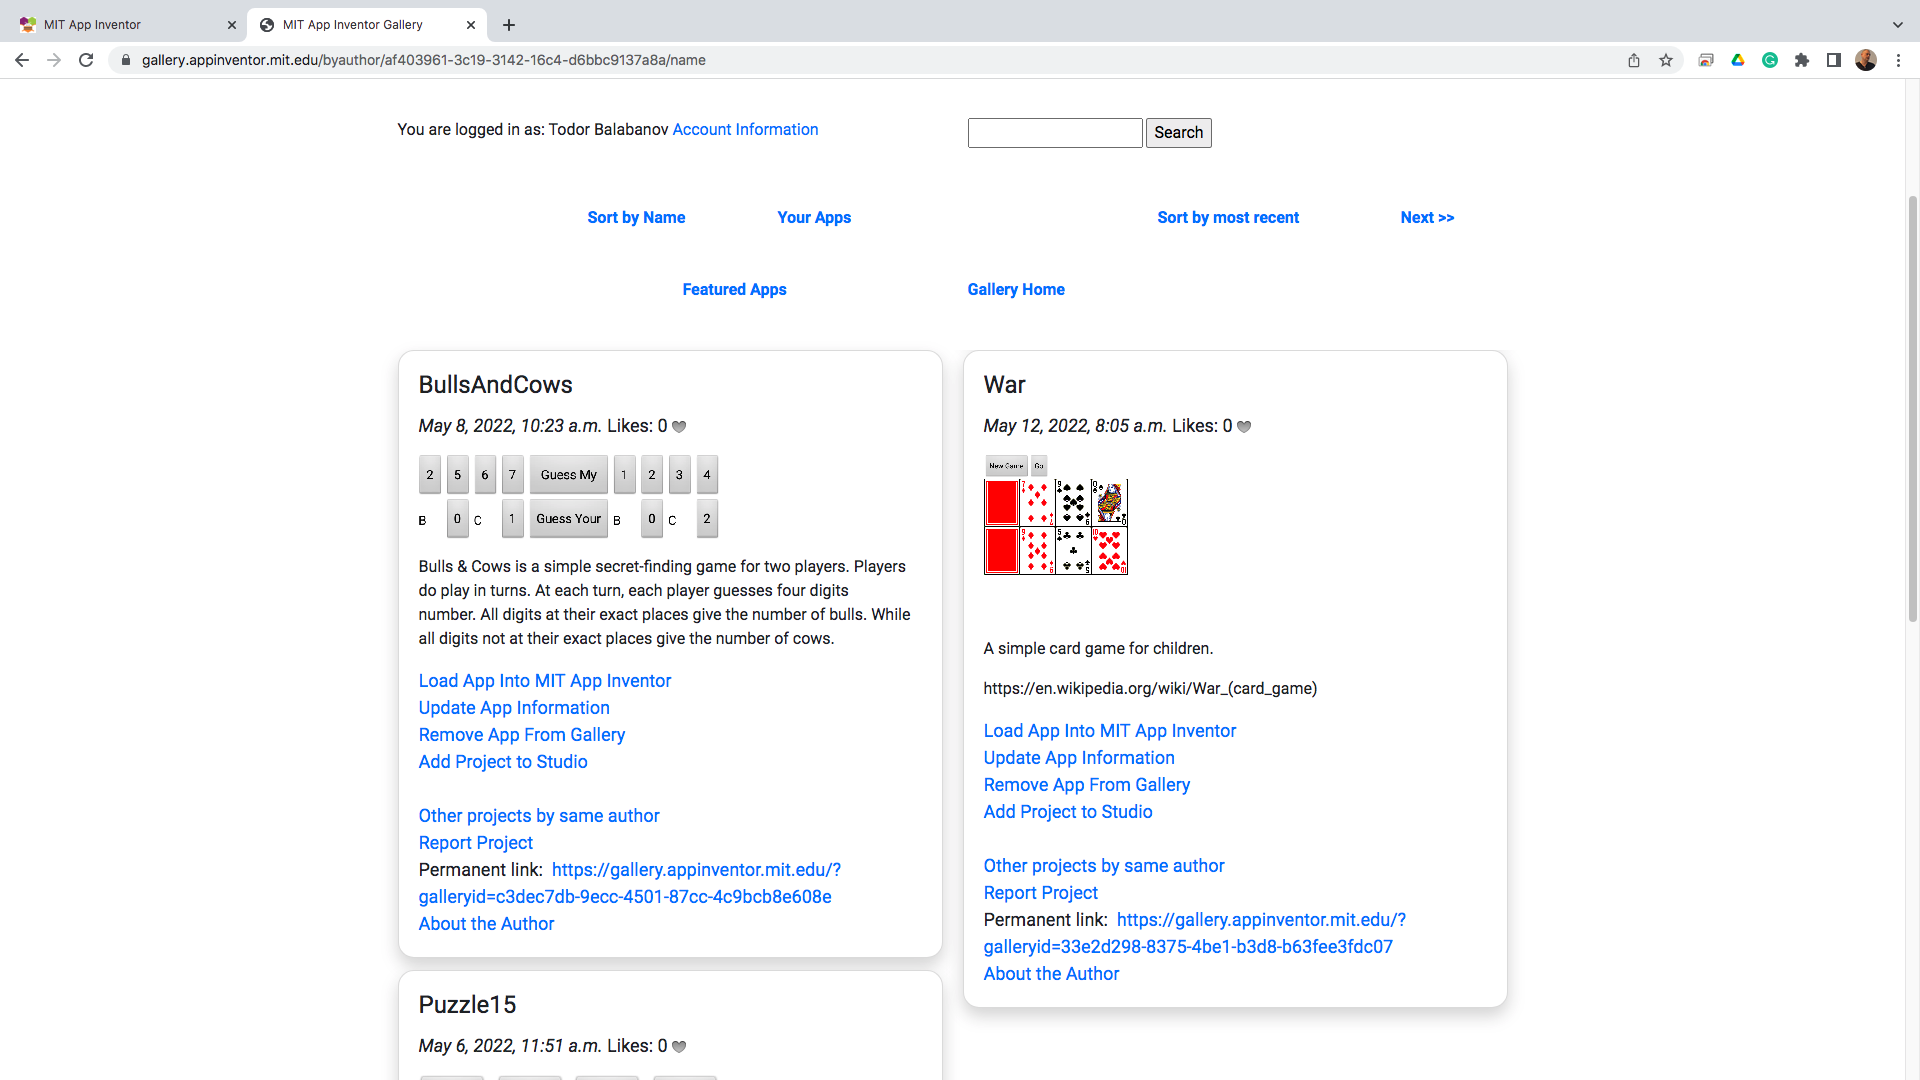
\includegraphics[width=1.0\linewidth,height=0.5\linewidth]{fig100030.png}
  \caption{Публикуване на играта за широката аудитория}
\label{fig100030}
\end{figure}

С това играта придобива своята първоначална завършеност. Разбира се, има още доста неща, които да се направят, така че от любителски проект да се превърне в софтуерен продукт за масова употреба. На първо място, може да се подобри визуализацията на картите и да се даде по-добра отчетност кой играч колко карти държи. Липсва помощна информация, както и оформление под формата на анимации при движението на картите. Тези подобрения излизат извън обхвата на настоящото изложение и остават за допълнително упражнение на читателите. 

